\documentclass{beamer}
\usepackage{etex}
\usepackage[utf8]{inputenc}

\usepackage{amsmath}
\usepackage{amsfonts}
\usepackage{amssymb}
\usepackage{amsthm}
\usepackage[ukrainian,russian]{babel}

\usepackage{fontenc}
\usepackage{graphicx}
\usepackage{wrapfig}
\usepackage{tikz}

\usepackage{ulem}

\usepackage{listings}
\usepackage{color}
\usepackage{hyperref}
% \usepackage[unicode,pdfusetitle, bookmarks=true, bookmarksnumbered=true,bookmarksopen=true,bookmarksopenlevel=1]{hyperref}
% \hypersetup{backref,colorlinks=true,linkcolor=blue,citecolor=green,bookmarks=false}
\usepackage{latexsym,url}
%  \bra and \ket are already defined in Qcircuit
% \usepackage{braket} 
\usepackage{multirow}

%    Q-circuit version 2
%    Copyright (C) 2004  Steve Flammia & Bryan Eastin
%    Last modified on: 9/16/2011
%
%    This program is free software; you can redistribute it and/or modify
%    it under the terms of the GNU General Public License as published by
%    the Free Software Foundation; either version 2 of the License, or
%    (at your option) any later version.
%
%    This program is distributed in the hope that it will be useful,
%    but WITHOUT ANY WARRANTY; without even the implied warranty of
%    MERCHANTABILITY or FITNESS FOR A PARTICULAR PURPOSE.  See the
%    GNU General Public License for more details.
%
%    You should have received a copy of the GNU General Public License
%    along with this program; if not, write to the Free Software
%    Foundation, Inc., 59 Temple Place, Suite 330, Boston, MA  02111-1307  USA

% Thanks to the Xy-pic guys, Kristoffer H Rose, Ross Moore, and Daniel Müllner,
% for their help in making Qcircuit work with Xy-pic version 3.8.  
% Thanks also to Dave Clader, Andrew Childs, Rafael Possignolo, Tyson Williams,
% Sergio Boixo, Cris Moore, Jonas Anderson, and Stephan Mertens for helping us test 
% and/or develop the new version.

\usepackage{xy}
\xyoption{matrix}
\xyoption{frame}
\xyoption{arrow}
\xyoption{arc}

\usepackage{ifpdf}
\ifpdf
\else
\PackageWarningNoLine{Qcircuit}{Qcircuit is loading in Postscript mode.  The Xy-pic options ps and dvips will be loaded.  If you wish to use other Postscript drivers for Xy-pic, you must modify the code in Qcircuit.tex}
%    The following options load the drivers most commonly required to
%    get proper Postscript output from Xy-pic.  Should these fail to work,
%    try replacing the following two lines with some of the other options
%    given in the Xy-pic reference manual.
\xyoption{ps}
\xyoption{dvips}
\fi

% The following resets Xy-pic matrix alignment to the pre-3.8 default, as
% required by Qcircuit.
\entrymodifiers={!C\entrybox}

\newcommand{\bra}[1]{{\left\langle{#1}\right\vert}}
\newcommand{\ket}[1]{{\left\vert{#1}\right\rangle}}
    % Defines Dirac notation. %7/5/07 added extra braces so that the commands will work in subscripts.
\newcommand{\qw}[1][-1]{\ar @{-} [0,#1]}
    % Defines a wire that connects horizontally.  By default it connects to the object on the left of the current object.
    % WARNING: Wire commands must appear after the gate in any given entry.
\newcommand{\qwx}[1][-1]{\ar @{-} [#1,0]}
    % Defines a wire that connects vertically.  By default it connects to the object above the current object.
    % WARNING: Wire commands must appear after the gate in any given entry.
\newcommand{\cw}[1][-1]{\ar @{=} [0,#1]}
    % Defines a classical wire that connects horizontally.  By default it connects to the object on the left of the current object.
    % WARNING: Wire commands must appear after the gate in any given entry.
\newcommand{\cwx}[1][-1]{\ar @{=} [#1,0]}
    % Defines a classical wire that connects vertically.  By default it connects to the object above the current object.
    % WARNING: Wire commands must appear after the gate in any given entry.
\newcommand{\gate}[1]{*+<.6em>{#1} \POS ="i","i"+UR;"i"+UL **\dir{-};"i"+DL **\dir{-};"i"+DR **\dir{-};"i"+UR **\dir{-},"i" \qw}
    % Boxes the argument, making a gate.
\newcommand{\meter}{*=<1.8em,1.4em>{\xy ="j","j"-<.778em,.322em>;{"j"+<.778em,-.322em> \ellipse ur,_{}},"j"-<0em,.4em>;p+<.5em,.9em> **\dir{-},"j"+<2.2em,2.2em>*{},"j"-<2.2em,2.2em>*{} \endxy} \POS ="i","i"+UR;"i"+UL **\dir{-};"i"+DL **\dir{-};"i"+DR **\dir{-};"i"+UR **\dir{-},"i" \qw}
    % Inserts a measurement meter.
    % In case you're wondering, the constants .778em and .322em specify
    % one quarter of a circle with radius 1.1em.
    % The points added at + and - <2.2em,2.2em> are there to strech the
    % canvas, ensuring that the size is unaffected by erratic spacing issues
    % with the arc.
\newcommand{\measure}[1]{*+[F-:<.9em>]{#1} \qw}
    % Inserts a measurement bubble with user defined text.
\newcommand{\measuretab}[1]{*{\xy*+<.6em>{#1}="e";"e"+UL;"e"+UR **\dir{-};"e"+DR **\dir{-};"e"+DL **\dir{-};"e"+LC-<.5em,0em> **\dir{-};"e"+UL **\dir{-} \endxy} \qw}
    % Inserts a measurement tab with user defined text.
\newcommand{\measureD}[1]{*{\xy*+=<0em,.1em>{#1}="e";"e"+UR+<0em,.25em>;"e"+UL+<-.5em,.25em> **\dir{-};"e"+DL+<-.5em,-.25em> **\dir{-};"e"+DR+<0em,-.25em> **\dir{-};{"e"+UR+<0em,.25em>\ellipse^{}};"e"+C:,+(0,1)*{} \endxy} \qw}
    % Inserts a D-shaped measurement gate with user defined text.
\newcommand{\multimeasure}[2]{*+<1em,.9em>{\hphantom{#2}} \qw \POS[0,0].[#1,0];p !C *{#2},p \drop\frm<.9em>{-}}
    % Draws a multiple qubit measurement bubble starting at the current position and spanning #1 additional gates below.
    % #2 gives the label for the gate.
    % You must use an argument of the same width as #2 in \ghost for the wires to connect properly on the lower lines.
\newcommand{\multimeasureD}[2]{*+<1em,.9em>{\hphantom{#2}} \POS [0,0]="i",[0,0].[#1,0]="e",!C *{#2},"e"+UR-<.8em,0em>;"e"+UL **\dir{-};"e"+DL **\dir{-};"e"+DR+<-.8em,0em> **\dir{-};{"e"+DR+<0em,.8em>\ellipse^{}};"e"+UR+<0em,-.8em> **\dir{-};{"e"+UR-<.8em,0em>\ellipse^{}},"i" \qw}
    % Draws a multiple qubit D-shaped measurement gate starting at the current position and spanning #1 additional gates below.
    % #2 gives the label for the gate.
    % You must use an argument of the same width as #2 in \ghost for the wires to connect properly on the lower lines.
\newcommand{\control}{*!<0em,.025em>-=-<.2em>{\bullet}}
    % Inserts an unconnected control.
\newcommand{\controlo}{*+<.01em>{\xy -<.095em>*\xycircle<.19em>{} \endxy}}
    % Inserts a unconnected control-on-0.
\newcommand{\ctrl}[1]{\control \qwx[#1] \qw}
    % Inserts a control and connects it to the object #1 wires below.
\newcommand{\ctrlo}[1]{\controlo \qwx[#1] \qw}
    % Inserts a control-on-0 and connects it to the object #1 wires below.
\newcommand{\targ}{*+<.02em,.02em>{\xy ="i","i"-<.39em,0em>;"i"+<.39em,0em> **\dir{-}, "i"-<0em,.39em>;"i"+<0em,.39em> **\dir{-},"i"*\xycircle<.4em>{} \endxy} \qw}
    % Inserts a CNOT target.
\newcommand{\qswap}{*=<0em>{\times} \qw}
    % Inserts half a swap gate.
    % Must be connected to the other swap with \qwx.
\newcommand{\multigate}[2]{*+<1em,.9em>{\hphantom{#2}} \POS [0,0]="i",[0,0].[#1,0]="e",!C *{#2},"e"+UR;"e"+UL **\dir{-};"e"+DL **\dir{-};"e"+DR **\dir{-};"e"+UR **\dir{-},"i" \qw}
    % Draws a multiple qubit gate starting at the current position and spanning #1 additional gates below.
    % #2 gives the label for the gate.
    % You must use an argument of the same width as #2 in \ghost for the wires to connect properly on the lower lines.
\newcommand{\ghost}[1]{*+<1em,.9em>{\hphantom{#1}} \qw}
    % Leaves space for \multigate on wires other than the one on which \multigate appears.  Without this command wires will cross your gate.
    % #1 should match the second argument in the corresponding \multigate.
\newcommand{\push}[1]{*{#1}}
    % Inserts #1, overriding the default that causes entries to have zero size.  This command takes the place of a gate.
    % Like a gate, it must precede any wire commands.
    % \push is useful for forcing columns apart.
    % NOTE: It might be useful to know that a gate is about 1.3 times the height of its contents.  I.e. \gate{M} is 1.3em tall.
    % WARNING: \push must appear before any wire commands and may not appear in an entry with a gate or label.
\newcommand{\gategroup}[6]{\POS"#1,#2"."#3,#2"."#1,#4"."#3,#4"!C*+<#5>\frm{#6}}
    % Constructs a box or bracket enclosing the square block spanning rows #1-#3 and columns=#2-#4.
    % The block is given a margin #5/2, so #5 should be a valid length.
    % #6 can take the following arguments -- or . or _\} or ^\} or \{ or \} or _) or ^) or ( or ) where the first two options yield dashed and
    % dotted boxes respectively, and the last eight options yield bottom, top, left, and right braces of the curly or normal variety.  See the Xy-pic reference manual for more options.
    % \gategroup can appear at the end of any gate entry, but it's good form to pick either the last entry or one of the corner gates.
    % BUG: \gategroup uses the four corner gates to determine the size of the bounding box.  Other gates may stick out of that box.  See \prop.

\newcommand{\rstick}[1]{*!L!<-.5em,0em>=<0em>{#1}}
    % Centers the left side of #1 in the cell.  Intended for lining up wire labels.  Note that non-gates have default size zero.
\newcommand{\lstick}[1]{*!R!<.5em,0em>=<0em>{#1}}
    % Centers the right side of #1 in the cell.  Intended for lining up wire labels.  Note that non-gates have default size zero.
\newcommand{\ustick}[1]{*!D!<0em,-.5em>=<0em>{#1}}
    % Centers the bottom of #1 in the cell.  Intended for lining up wire labels.  Note that non-gates have default size zero.
\newcommand{\dstick}[1]{*!U!<0em,.5em>=<0em>{#1}}
    % Centers the top of #1 in the cell.  Intended for lining up wire labels.  Note that non-gates have default size zero.
\newcommand{\Qcircuit}{\xymatrix @*=<0em>}
    % Defines \Qcircuit as an \xymatrix with entries of default size 0em.
\newcommand{\link}[2]{\ar @{-} [#1,#2]}
    % Draws a wire or connecting line to the element #1 rows down and #2 columns forward.
\newcommand{\pureghost}[1]{*+<1em,.9em>{\hphantom{#1}}}
    % Same as \ghost except it omits the wire leading to the left. 

\newcommand {\Had} {H}%{\mbox{\sf{H}}}
\newcommand {\phase} {S}%{\mbox{\sf{S}}}
\newcommand {\R} {R_3}%{\mbox{\sf{R}}_3}
\newcommand {\cnot} {\textit{cnot}\,}%{\mbox{\sf{cnot}}}
\newcommand {\X} {X}%{\mbox{\sf{X}}}
\newcommand {\Y} {Y}%{\mbox{\sf{Y}}}
\newcommand {\Z} {Z}%{\mbox{\sf{Z}}}


\usetheme{Warsaw}
\author{Ширай Андрей}
 \institute{}
\title{Квантовая информатика -- что, зачем и почему?}
\date{\today}

\newtheorem{defin}{Определение}
\newtheorem{theor}{Теорема}
\newtheorem{astat}{}
\newtheorem{stat}{Постулат}



\begin{document}
\frame{\titlepage}

\frame{
\frametitle{We have a plan!}

\begin{itemize}
 \item Исторический экскурс.
 \item Как это работает.
 \item Примеры физических реализаций.
 \item Квантовые алгоритмы Шора(факторизация) и Гровера(поиск по неупорядоченной БД).
 \item Как это повлияет на надежность криптосистем?
 \item Как квантовая информатика повлияла на другие направления теоретической 
информатики/математики/физики.
 \item Моделирование квантовых вычислений
\end{itemize}

}

% % % % % % % % % % % % % % 


\frame{
\frametitle{Вы, конечно же шутите, мистер Фейнман!}
\begin{center}
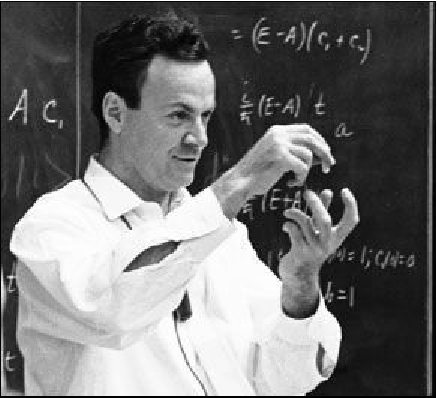
\includegraphics[scale=0.7]{f.pdf}


Feynman, R. P. (1982). \textit{"Simulating physics with computers"}. International Journal of Theoretical Physics 21 (6): 467–488. 

\end{center}


}

% % % % % % % % % % % % % % 

\frame{

\frametitle{Освой линейную алгебру за 240 секунд!}

\[
\begin{pmatrix}\frac{1}{2} & 0 \cr 0 & \frac{1}{2}\end{pmatrix}
\begin{pmatrix}1\cr 0 \end{pmatrix} =
\begin{pmatrix}\frac{1}{2}\cr 0 \end{pmatrix}
\]

\begin{center}
\begin{tabular}{ll}
\begin{tikzpicture}[scale=2]
% \clip (-4.63205,-1.88345) rectangle (4.06915,1.88345);
\draw [step=.1cm, help lines] (0,0) grid (1,1);
\draw [help lines] (-1,0) grid (0,1);
\draw [help lines] (0,-1) grid (1,0);
\draw [help lines] (-1,-1) grid (0,0);
\draw [color=black,->] (-1,0) -- (1,0);
\draw [color=black,->] (0,-1) -- (0,1);
%% вектор;
\draw[blue, line width=1pt, solid, ->] (0,0) -- (1,0);

\end{tikzpicture} & 
\begin{tikzpicture}[scale=2]
% \clip (-4.63205,-1.88345) rectangle (4.06915,1.88345);
\draw [step=.1cm,help lines] (0,0) grid (1,1);
\draw [help lines] (-1,0) grid (0,1);
\draw [help lines] (0,-1) grid (1,0);
\draw [help lines] (-1,-1) grid (0,0);
\draw [color=black,->] (-1,0) -- (1,0);
\draw [color=black,->] (0,-1) -- (0,1);
%% вектор;
\draw[blue, line width=1pt, solid, ->] (0,0) -- (0.5,0);

\end{tikzpicture} 
\end{tabular}
\end{center}

}

\frame{

\frametitle{Освой линейную алгебру за 240 секунд!}
\[
\begin{pmatrix}\frac{1}{\sqrt{2}} & \frac{1}{\sqrt{2}}\cr \frac{1}{\sqrt{2}} & -\frac{1}{\sqrt{2}}\end{pmatrix}
\begin{pmatrix}1\cr 0\end{pmatrix} =
\begin{pmatrix}\frac{1}{\sqrt{2}}\cr \frac{1}{\sqrt{2}}\end{pmatrix}
\]

\begin{center}
\begin{tabular}{ll}
\begin{tikzpicture}[scale=2]
% \clip (-4.63205,-1.88345) rectangle (4.06915,1.88345);
\draw [step=.1cm,help lines] (0,0) grid (1,1);
\draw [help lines] (-1,0) grid (0,1);
\draw [help lines] (0,-1) grid (1,0);
\draw [help lines] (-1,-1) grid (0,0);
\draw [color=black,->] (-1,0) -- (1,0);
\draw [color=black,->] (0,-1) -- (0,1);
%% вектор;
\draw[blue, line width=1pt, solid, ->] (0,0) -- (1,0);

\end{tikzpicture} & 
\begin{tikzpicture}[scale=2]
% \clip (-4.63205,-1.88345) rectangle (4.06915,1.88345);
\draw [step=.1cm,help lines] (0,0) grid (1,1);
\draw [help lines] (-1,0) grid (0,1);
\draw [help lines] (0,-1) grid (1,0);
\draw [help lines] (-1,-1) grid (0,0);
\draw [color=black,->] (-1,0) -- (1,0);
\draw [color=black,->] (0,-1) -- (0,1);
%% вектор;
\draw[blue, line width=1pt, solid, ->] (0,0) -- (0.707,0.707);

\end{tikzpicture} 
\end{tabular}
\end{center}
}




\frame{
\frametitle{Стохастические вычисления}

\begin{center}
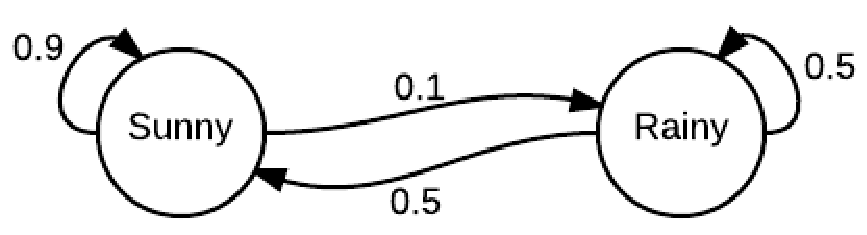
\includegraphics[scale=0.5]{mar.pdf}
\end{center}


$P= \begin{pmatrix}0.9 & 0.5\cr 0.1 & 0.5\end{pmatrix}$ --матрица перехода для некоторой цепи Маркова.
Входные данные: $x=\begin{pmatrix}1\cr 0\end{pmatrix}$ -- у нас хорошая погода.
\[
\begin{pmatrix}0.9 & 0.5\cr 0.1 & 0.5\end{pmatrix}
\begin{pmatrix}1\cr 0\end{pmatrix} =
\begin{pmatrix}0.9\cr 0.1\end{pmatrix}
\]
-- с вероятностью 10\% завтра пойдет дождь.

Неподвижная точка  $\approx \begin{pmatrix}0.833\cr 0.167\end{pmatrix}$



}


% % % % % % % % % % % % % % 

\frame{

\frametitle{Квантовая механика одним слайдом}
\begin{center}
\begin{tabular}{c|c}
Стохастика & ``Кванты'' \\ 
$ \begin{pmatrix}
s_{11} & \dots &s_{1n}\\ 
\vdots & \ddots & \vdots \\ 
s_{n1} & \dots & s_{nn}
\end{pmatrix}
\begin{pmatrix}
p_1\\ 
\vdots \\ 
p_n
\end{pmatrix}
=
\begin{pmatrix}
q_1\\ 
\vdots \\ 
q_n
\end{pmatrix}$ &
$ \begin{pmatrix}
u_{11} & \dots & u_{1n}\\ 
\vdots & \ddots & \vdots \\ 
u_{n1} & \dots & u_{nn}
\end{pmatrix}
\begin{pmatrix}
\alpha_1\\ 
\vdots \\ 
\alpha_n
\end{pmatrix}
=
\begin{pmatrix}
\beta_1\\ 
\vdots \\ 
\beta_n
\end{pmatrix}$ \\
$ p_i \geq 0, \sum_{i=1}^{n} p_i =1 $ & $ \alpha \in \mathbb{C},  \sum_{i=1}^{n}\left \| \alpha_i \right \|^2 =1  $
\end{tabular}
\smallskip



Сформулировано страшно коряво, в каком-то смысле даже неверно, но зато правильно и понятно. \copyright


\end{center}

}


\frame{

\frametitle{Гильбертово пространство}
\begin{stat}
 Физическое состояние замкнутой квантовой системы описывается  нормированным вектором состояния $\ket{\psi}$ в линейном комплексном пространстве с внутреним произведением(Гильбертовом пространстве)
\end{stat}

\begin{stat}
 Динамическая эволюция замкнутой квантовой системы описывается \textit{унитарным} преобразованием:
 \[
  \ket{\psi(t)} = \hat{U}(t) \ket{\psi(0)} 
 \]

\end{stat}
}

\frame{
\frametitle{Суперпозиция}
\begin{astat}
% Возможно, для прогресса в понимании таких явлений намнедостает математической теории квантовых автоматов Такие объекты могли бы показать нам математические модели детерминированных процессов с совершенно непривычными свойствами. 
 ... Одна из причин этого в том, что квантовое пространство состояний обладает гораздо большей емкостью, чем классическое: там, где в классике имеется N дискретных состояний, в квантовой теории, допускающей их суперпозицию, имеется $c^N$ планковских ячеек. При объединении классических систем их числа состояний $N_1$ и $N_2$ перемножаются, а в квантовом варианте получается $c^{N_1 N_2}$.
\end{astat}
Ю. Манин \textit{``Вычислимое и невычислимое''}

% \begin{astat}
%  \[
%   \ket{ \psi } = \alpha_0 \ket{0} + \alpha_1 \ket{1}
%  \]
%  
% \[
%  \sum \left \| \alpha_i \right \|^2 =1
% \]
% 
% \end{astat}


}

\frame{
\frametitle{Коллапс}
% Возможно, для прогресса в понимании таких явлений намнедостает математической теории квантовых автоматов Такие объекты могли бы показать нам математические модели детерминированных процессов с совершенно непривычными свойствами. 
... Одна из причин этого в том, что квантовое пространство состояний обладает гораздо большей емкостью, чем классическое: там, где в классике имеется N дискретных состояний, в квантовой теории, допускающей их суперпозицию, имеется $c^N$ планковских ячеек. При объединении классических систем их числа состояний $N_1$ и $N_2$ перемножаются, а в квантовом варианте получается $c^{N_1 N_2}$.


\begin{stat}
 При измерении наблюдаемой $A$ ее состояние редуцируется в один из векторов оператора $\hat{A}$
\end{stat}



}

\frame{
\frametitle{Измерение и наблюдаемые}

\begin{stat}
 При измерении наблюдаемой $A$ ее состояние редуцируется в один из собственных векторов оператора $\hat{A}$
\end{stat}

\begin{center}
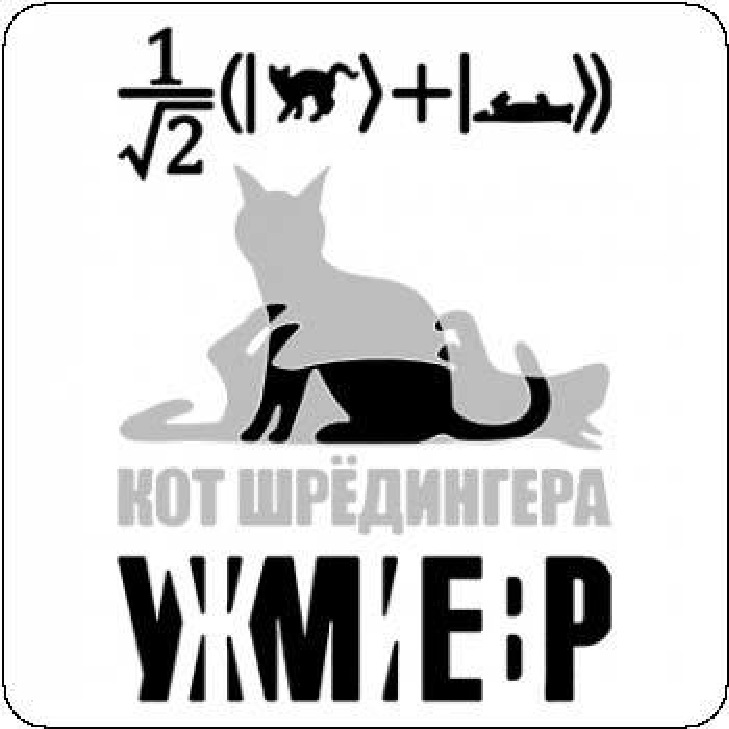
\includegraphics[scale=0.45]{sc.pdf}
\end{center}

}

\frame{
\frametitle{Продвинутый курс линейной алгебры для чайников}

\begin{defin}
 \textbf{Cобственный вектор} -- любой ненулевой вектор $\vec{x}$, который отображается оператором в коллинеарный $\lambda \vec{x}$, а соответствующий скаляр $\lambda$ называется \textit{собственным значением} оператора.
\end{defin}

\[
\begin{pmatrix}\frac{1}{\sqrt{2}} & \frac{1}{\sqrt{2}}\cr \frac{1}{\sqrt{2}} & -\frac{1}{\sqrt{2}}\end{pmatrix}
\begin{pmatrix}1\cr -\sqrt{2}-1\end{pmatrix} =
\begin{pmatrix}-1\cr \sqrt{2}+1\end{pmatrix}
\]

\begin{center}
\begin{tabular}{ll}
\begin{tikzpicture}[scale=1]
% \clip (-4.63205,-1.88345) rectangle (4.06915,1.88345);
\draw [step=.1cm,help lines] (0,0) grid (1,1);
\draw [help lines] (-1,0) grid (0,1);
\draw [help lines] (0,-1) grid (1,0);
\draw [help lines] (-1,-1) grid (0,0);
\draw [color=black,->] (-1,0) -- (1,0);
\draw [color=black,->] (0,-1) -- (0,1);
%% вектор;
\draw[blue, line width=1pt, solid, ->] (0,0) -- (1,0);
% \draw[red, line width=1pt, solid, ->] (0,0) -- (1,-2.414);
\draw[red, line width=1pt, solid, ->] (0,0) -- (1/2.6131259,-2.414/2.6131259 );
\end{tikzpicture} & 
\begin{tikzpicture}[scale=1]
% \clip (-4.63205,-1.88345) rectangle (4.06915,1.88345);
\draw [step=.1cm,help lines] (0,0) grid (1,1);
\draw [help lines] (-1,0) grid (0,1);
\draw [help lines] (0,-1) grid (1,0);
\draw [help lines] (-1,-1) grid (0,0);
\draw [color=black,->] (-1,0) -- (1,0);
\draw [color=black,->] (0,-1) -- (0,1);
%% вектор;
\draw[blue, line width=1pt, solid, ->] (0,0) -- (0.707,0.707);
% \draw[red, line width=1pt, solid, ->] (0,0) -- (-1,2.414);
\draw[red, line width=1pt, solid, ->] (0,0) -- (-1/2.6131259,2.414/2.6131259);
\end{tikzpicture} 
\end{tabular}
\end{center}



}



\frame{
\frametitle{Операторы}
\begin{defin}
 Оператор $\hat{P}$, для которого $\hat{P}^2 = \hat{P}$ называется \textbf{проектором}.
\end{defin}
\begin{center}
% \begin{tabular}{c|c}
% \begin{tikzpicture}[scale=2]
%  % \clip (-4.63205,-1.88345) rectangle (4.06915,1.88345);
% % \draw [help lines] (0,0) grid (1,1);
% % \draw [help lines] (-1,0) grid (0,1);
% % \draw [help lines] (0,-1) grid (1,0);
% % \draw [help lines] (-1,-1) grid (0,0);
% \draw [color=black,->] (-1,0) -- (1,0);
% \draw [color=black,->] (0,-1) -- (0,1);
% %% вектор;
% \draw[blue, line width=1pt, solid, ->] (0,0) -- (0.707,0.707);
% \draw[red, dashed] (0.707,0.707) -- (0.707,0);
% 
% \node (X) at (1.2,0) {$\ket{0}$};
% \node (Y) at (0,1.1) {$\ket{1}$};
% \node (P) at (0.85,0.85) {$\ket{\psi}$};
% \end{tikzpicture}
% & $\|x\|^2=\sum_{k=1}^{\infty}\left|\langle x,e_k\rangle\right|^2.$
% \end{tabular}
% Равенство Парсеваля: $\|x\|^2=\sum_{k=1}^{\infty}\left|\langle x,e_k\rangle\right|^2$
\begin{tabular}{cc}
\multirow{5}{*}{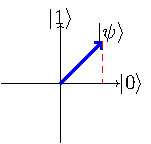
\includegraphics[scale=1.8]{p.pdf}} &  \\
% \cline{2-2} 
& \\
& \\
& \\
 &  \\
\end{tabular}
\end{center}
}


\frame{
\frametitle{Сфера Блоха}

% \begin{center}
\begin{tabular}{cc}
\multirow{5}{*}{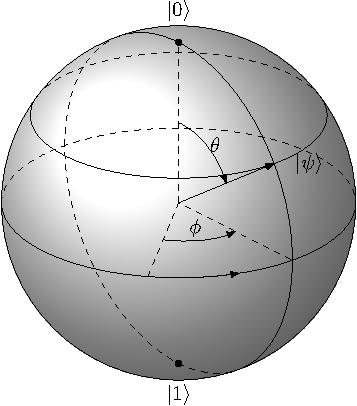
\includegraphics[scale=0.7]{bloch.pdf}} &  $ \ket{\psi}=\alpha\ket{0}+\beta\ket{1} = \begin{pmatrix}\alpha\cr \beta\end{pmatrix}$ \\
% \cline{2-2} 
& \\
& $ \left \| \alpha \right \|^2 + \left \| \beta \right \|^2=1 $\\
& \\
 &  $\ket{\psi}=e^{-i\phi/2}\cos\frac{\theta}{2}\ket{0} + e^{i\phi/2}\sin\frac{\theta}{2}\ket{1}$ \\
\end{tabular}

% \begin{tabular}{cc}
%  \multirow{2}{*}{} & $ \ket{\psi}=\alpha\ket{0}+\beta\ket{1} = \begin{pmatrix}\alpha\cr \beta\end{pmatrix}$  
% \cline{2-2} 
% & $\ket{\psi}=e^{-i\phi/2}\cos\frac{\theta}{2}\ket{0} + e^{i\phi/2}\sin\frac{\theta}{2}\ket{1}$
% 
% \end{tabular}
% \end{center}
}


\frame{
\frametitle{ЭПР-парадокс}
\begin{center}
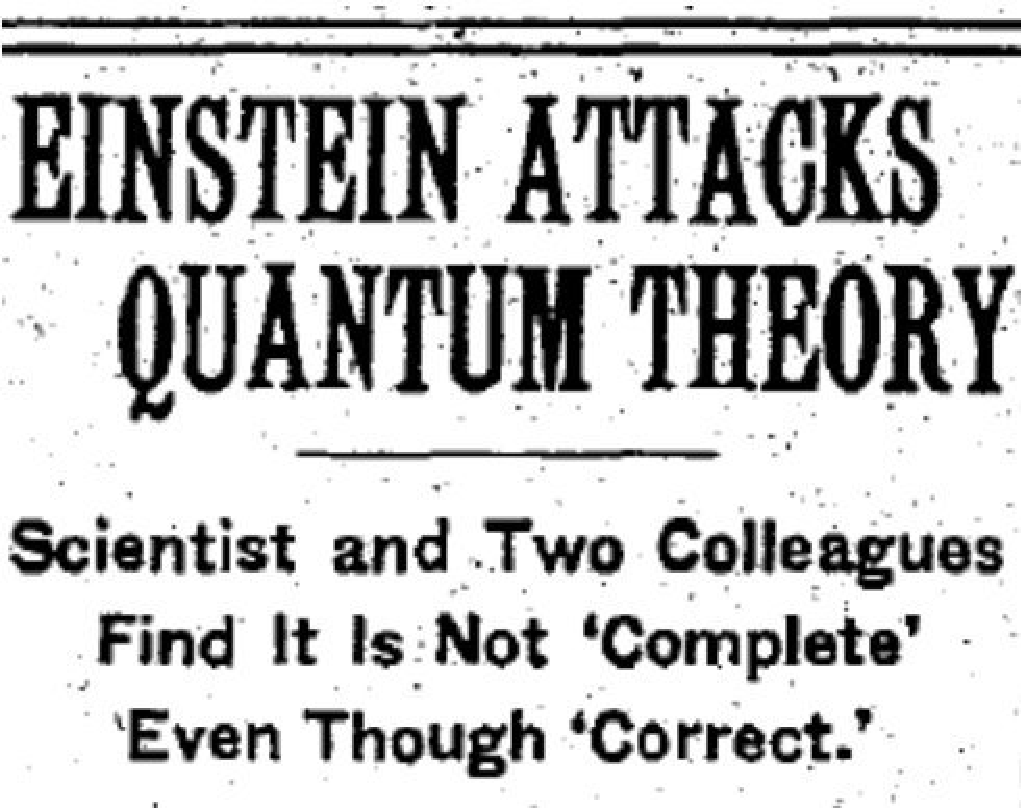
\includegraphics[scale=0.5]{Einstein_attacks.pdf}
\end{center}
}


\frame{
\frametitle{Запутаность}

Сепарабельное состояние:
\begin{equation}
   (\alpha\ket{0} + \beta\ket{1}) \otimes (\gamma\ket{0} + \delta\ket{1}) = 
   \alpha\gamma\ket{00} + \alpha\delta\ket{01} +\beta\gamma\ket{10} +\beta\delta\ket{11} 
\end{equation}

Несепарабельное состояние:
\begin{equation}
 \frac{\ket{00}+\ket{11}}{\sqrt{2}}
\end{equation}

}


\frame{

\frametitle{Квантовые схемы}
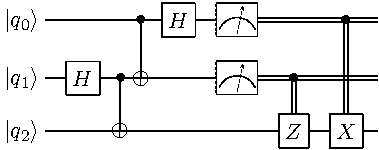
\includegraphics[scale=1.5]{test2.pdf}
}
\frame{
\frametitle{Квантовые схемы}
\begin{center}
\begin{tabular}[c]{c|c|c}
$\X$ & $\begin{pmatrix}0 & 1\cr 1 & 0\end{pmatrix}$ & $\X\ket{0} = \ket{1}$\\
& & $\X \ket{1} = \ket{0}$ \\ \hline
& & \\ 
$\Z$ & $\begin{pmatrix}1 & 0\cr 0 & -1\end{pmatrix}$ & $\Z\ket{0} = \ket{0}$\\
& & $\Z\ket{1} = -\ket{1}$ \\ \hline
& & \\ 
$\Had$ & $\begin{pmatrix}\frac{1}{\sqrt{2}} & \frac{1}{\sqrt{2}}\cr \frac{1}{\sqrt{2}} & -\frac{1}{\sqrt{2}}\end{pmatrix}$ & $\Had\ket{0} = \ket{+} = \frac{1}{\sqrt{2}}(\ket{0}+\ket{1})$ \\
& & $\Had\ket{1} = \ket{-} = \frac{1}{\sqrt{2}}(\ket{0}-\ket{1})$
\end{tabular}
\end{center}


}
\frame{

\frametitle{Квантовые схемы}
\begin{center}
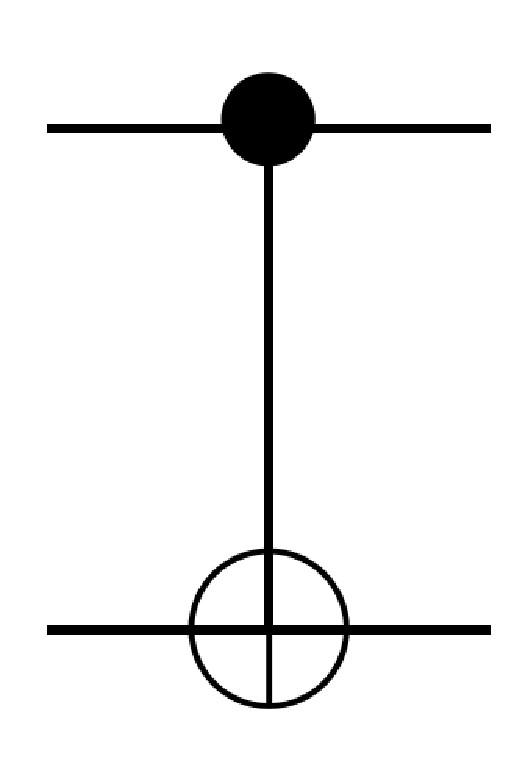
\includegraphics[scale=0.25]{cnot.pdf} 
\end{center}
% \[
% \begin{pmatrix}1 & 0 & 0 & 0\cr 0 & 1 & 0 & 0\cr 0 & 0 & 0 & 1\cr 0 & 0 & 1 & 0\end{pmatrix}
% \]


\begin{align*}
\ket{00} \to \ket{00}  \\ 
\ket{01} \to \ket{00}\\ 
\ket{10} \to \ket{11} \\ 
\ket{11} \to \ket{10}
\end{align*}

}
% \frame{
% 
% \frametitle{Квантовые схемы}
% 
% }
% 
% 
% \frame{
% 
% \frametitle{Квантовые схемы -- обратимость}
% 
% }

% % % % % % % % % % % % % % 

\frame{
\frametitle{Джозефсоновские кубиты}
\begin{center}
 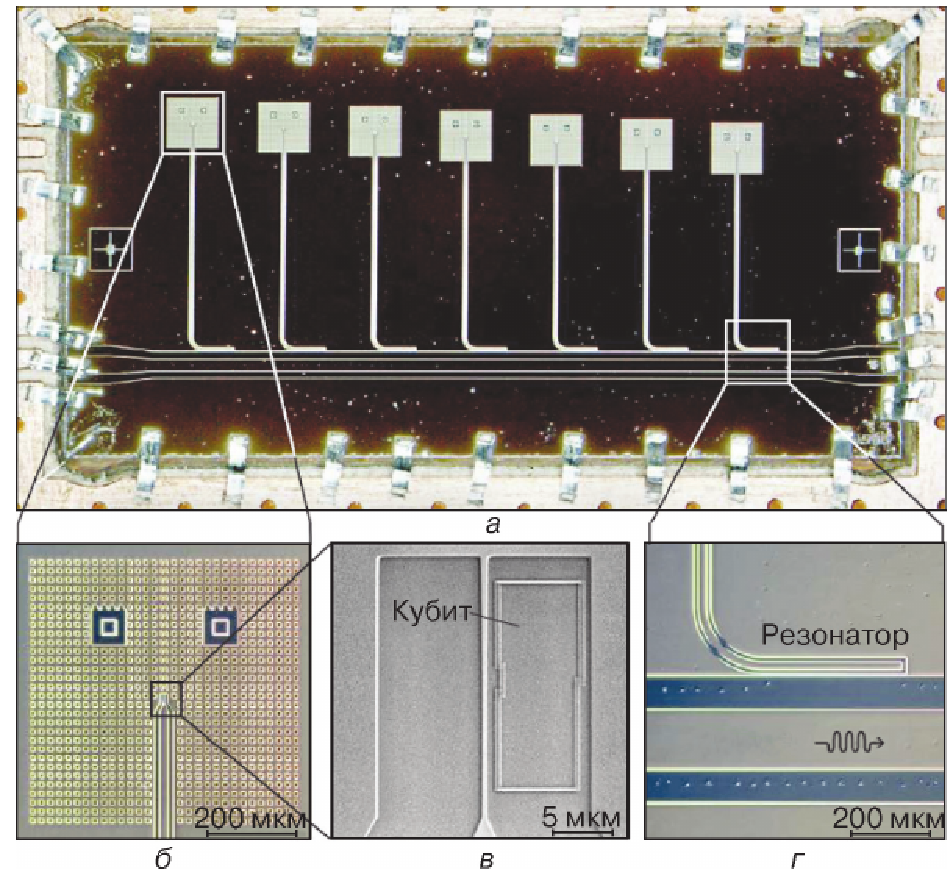
\includegraphics[scale=0.4]{q_jj.pdf}

\end{center}
\tiny M. Jerger, S. Poletto, P. Macha, U. Hübner, A. Lukashenko, E. Il’ichev, A. V. Ustinov \textit{Readout of a qubit array via a single transmission line}, Europhys. Lett. 96, (2011) 40012
}


% \frame{
% \frametitle{Джозефсоновские кубиты}
% \begin{center}
% 
%  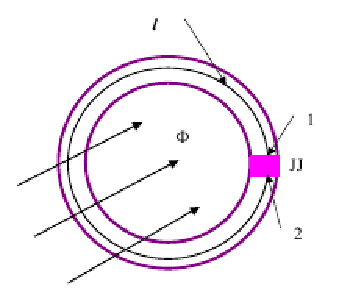
\includegraphics[scale=1]{jj.pdf} 
%  
% 
% \end{center}
% }

\frame{
\frametitle{D-Wave}
\begin{center}
 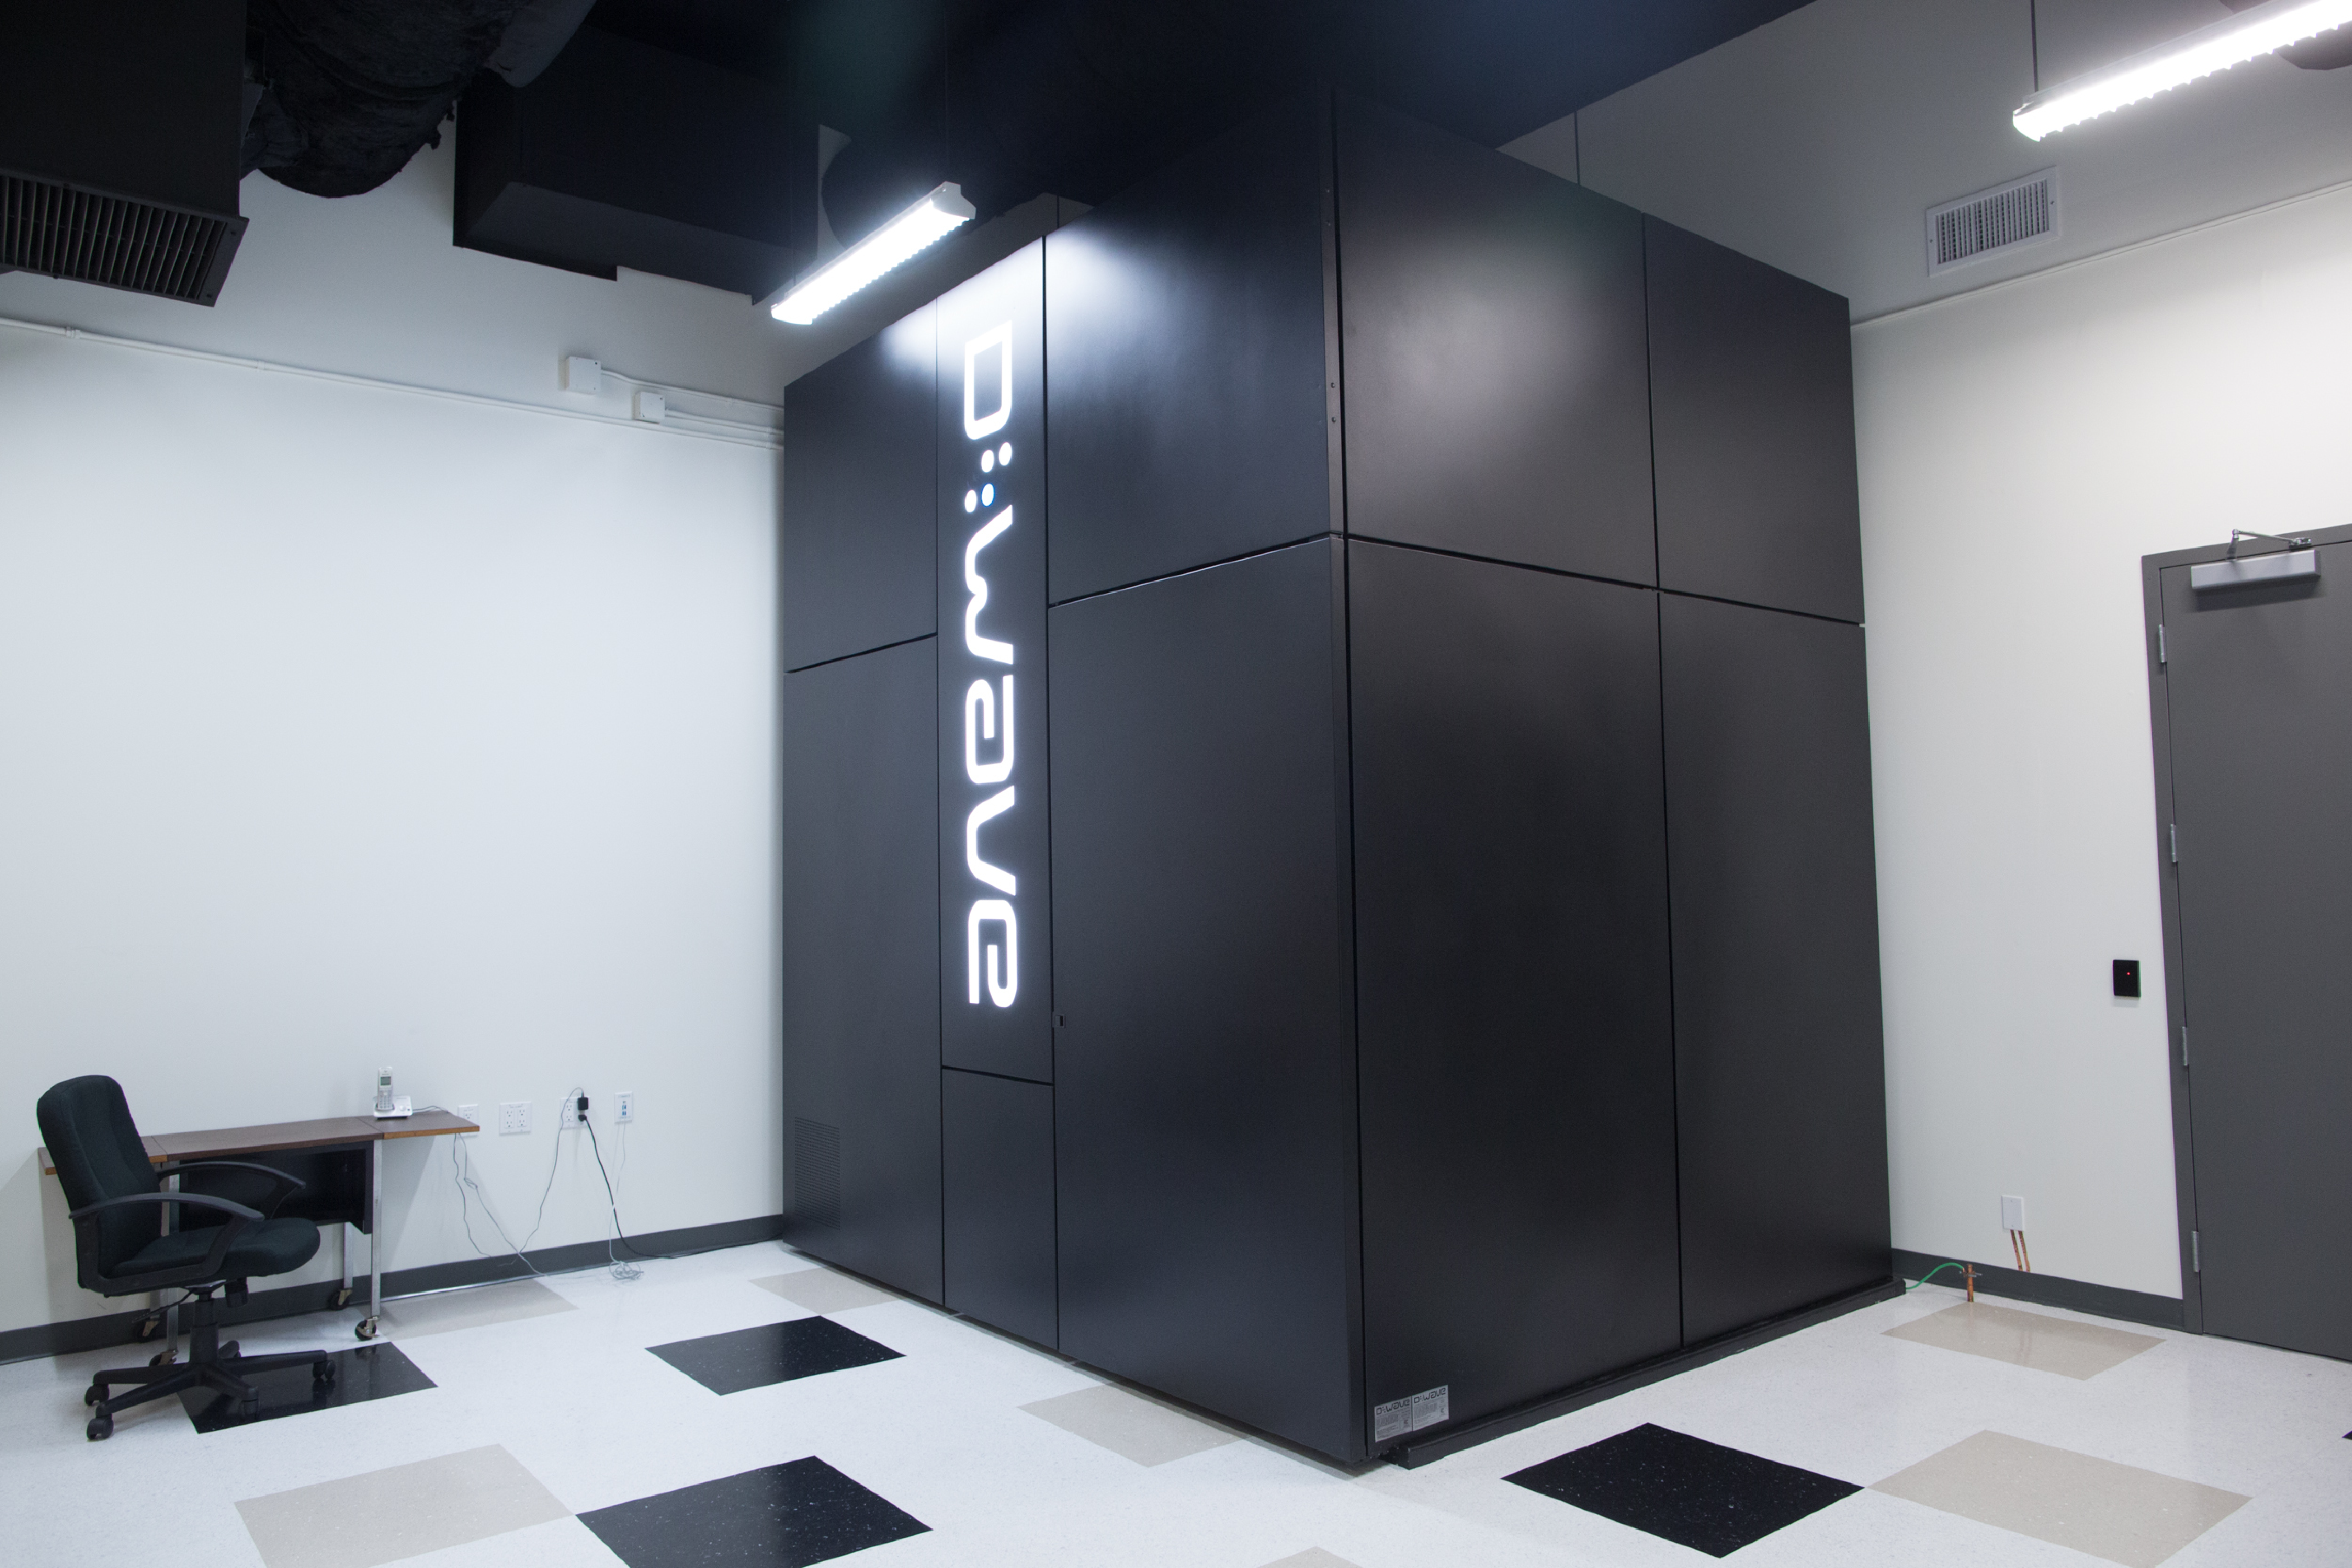
\includegraphics[scale=0.1]{dw.pdf}
 
\tiny
Sergio Boixo, Troels F. Rønnow, Sergei V. Isakov, Zhihui Wang, David Wecker, Daniel A. Lidar, John M. Martinis, Matthias Troyer  \textit{Quantum annealing with more than one hundred qubits},  	arXiv:1304.4595 
\end{center}
}

% % % % % % % % % % % % % % 
\frame{
\frametitle{Алгоритм Гровера}
Сначала формируют равномернe суперпозицию всех состояний: $\operatorname{H}^{\otimes n}\ket{0} = \frac{1}{\sqrt{N}}\sum_x\ket{x}$. Чуть дальше будет обозначать для краткости равномерную суперпозицию как $\ket{\psi}$ Потом последовательно применяется оператор Гровера: 
\begin{enumerate}
 \item К входу применяется оракул $O$: $\ket{x} \to (-1)^{f(x)} \ket{x} $ Т.е. это единичная матрица, где на месте ответов стоят -1. \footnote{Очевидно, что $O^2=I$, так что унитарность сохраняется.}
 \item Опять преобразование Адамара $\operatorname{H}^{\otimes n}$
 \item Условный сдвиг фазы: $\ket{x} \to -(-1)^{\delta_{0x}\ket{x}}$, этой операции соответствует унитарный оператор $\ket{0}\bra{0}-I$.
%  Это тоже унитарная операция: $(\frac{2}{N} - 1)^2 + (N-1)(\frac{2}{N})^2 = \frac{4}{N^2} - \frac{4}{N} + 1 + \frac{4}{N} - \frac{4}{N^2} = 1$ 
 \item Опять преобразование Адамара $\operatorname{H}^{\otimes n}$
\end{enumerate}
\[
 G =  (\ket{\psi}\bra{\psi}-I)O
\]

}

\frame{
\frametitle{Алгоритм Гровера}
\begin{align*}
 \Qcircuit @C=1em @R=.7em {
                   &         &                      &                         &                      & \ustick{\text{Оператор Гровера G:}} \\
  \lstick{\ket{0}} & /^n \qw & \gate{H^{\otimes n}} & \multigate{1}{O} & \gate{H^{\otimes n}} & \gate{2 \ket{\psi}\bra{\psi} - I_n}         & \gate{H^{\otimes n}} & \qw & \cdots & & \meter & \cw \\
  \lstick{\ket{1}} & \qw     & \gate{H}             & \ghost{O}        & \qw                  & \qw                                       & \qw                  & \qw & \cdots & \\
                   &         &                      &                         &                      & \dstick{\text{Выполняется $O(\sqrt{N})$ раз}}
  \gategroup{2}{5}{2}{7}{.7em}{^\}}
  \gategroup{2}{4}{3}{10}{.7em}{_\}}
 }
\end{align*}


}

\frame{
\frametitle{Геометрическая интерпритация алгоритма Гровера}
% Физический смысл оператора G довольно простост -- это вращение в двухмерном пространстве, порождаемом вектором $\ket{\psi}$ и ветором-решением. 
Мы можем переписать $\ket{\psi}$, как:
\[
 \ket{\psi} = \sqrt{\frac{N-M}{N}} \ket{\alpha} + \sqrt{\frac{M}{N}}\ket{\beta}=\cos{\frac{\theta}{2}}\ket{\alpha} + \sin{\frac{\theta}{2}}\ket{\beta}
\]
,где $\ket{\alpha}=\frac{1}{\sqrt{N-M}}\sum_{\neg f(x)}\ket{x}$ и $\ket{\beta}=\frac{1}{\sqrt{M}}\sum_{f(x)}\ket{x}$



\begin{center}
\begin{tikzpicture}[scale=2]
 % \clip (-4.63205,-1.88345) rectangle (4.06915,1.88345);
% \draw [help lines] (0,0) grid (1,1);
% \draw [help lines] (-1,0) grid (0,1);
% \draw [help lines] (0,-1) grid (1,0);
% \draw [help lines] (-1,-1) grid (0,0);
\draw [color=black,->] (-1,0) -- (1,0);
\draw [color=black,->] (0,-1) -- (0,1);
%% вектор;
\draw[red, line width=1pt, solid, ->] (0,0) -- (0.75,0.25);
\draw[green, line width=1pt, solid, ->] (0,0) -- (0.75,-0.25);
\draw[blue, line width=1pt, solid, ->] (0,0) -- (0.25,0.75);

\draw[lightgrey, dashed] (0.75,0.25) -- (0.75,-0.25);
\draw[darkgrey, dashed] (0.75,-0.25) -- (0.25,0.75);

\node (X) at (1.2,0) {$\ket{\alpha}$};
\node (Y) at (0,1.1) {$\ket{\beta}$};
\node (P) at (0.85,0.35) {$\ket{\psi}$};
\node (P2) at (0.85,-0.35) {$\operatorname{O}\ket{\psi}$};
\node (P3) at (0.35,0.85) {$\operatorname{G}\ket{\psi}$};
\end{tikzpicture}
% \includegraphics[scale=0.45]{grvr.pdf}
\end{center}

}


\frame{
\frametitle{Оптимальность алгоритма Гровера...}
% \[
%  G\ket{\psi} = \cos{\frac{3\theta}{2}}\ket{\alpha} + \sin{\frac{3\theta}{2}}\ket{\beta}
% \]
\[
 G^k \ket{\psi} = \cos{\frac{(2k+1)\theta}{2}}\ket{\alpha} + \sin{\frac{(2k+1)\theta}{2}}\ket{\beta}
\]
И необходимое количество итераций:
\[
 R = \lfloor \arcsin{\frac{\sqrt{M/N}}{\theta}} \rfloor \stackrel{M \leq N/2}{=} \lfloor \frac{\pi}{4} \sqrt{\frac{N}{M}} \rfloor
\]
\begin{theor}
 Алгоритм Гровера -- оптимальный
\end{theor}
% Идея доказательства состоит в оценке $D_k$ -- меры отклонения оракулом после $k$ вызовов. Она растет не быстрее, чем $O(k^2)$ и имеет порядок $\Omega(N)$, откуда будет следовать, что необходимо не меньше  $\Omega(\sqrt{N})$ обращений к оракулу. 
% \[
%  O(\sqrt{N}) \wedge \Omega(\sqrt{N}) \Rightarrow \Theta(\sqrt{N})
% \]

}
\frame{
\frametitle{Оптимальность алгоритма Гровера... или почему $\mathcal{P}\neq\mathcal{NP} $}
\begin{enumerate}
 \item Линейность\footnote{В смысле линейность \textbf{интегрального оператора}, а не подинтегрального выражения!} квантовой механики $\rightarrow$ Предел Гровера $\sqrt{N}$
\item А если у нас будут нелинейные квантовые операторы, сохраняющие нормировку? (``Приличная'' нелинейная КМ)
\end{enumerate}
}



\frame{
\frametitle{Оптимальность алгоритма Гровера... или почему $\mathcal{P}\neq\mathcal{NP} $}
\begin{enumerate}
 \item Линейность квантовой механики $\rightarrow$ Предел Гровера $\sqrt{N}$
\item Нелинейная КМ передает сигналы быстрее с и  решает $\mathcal{\#P}$-полные проблемы за полиномиальное время!\footnote{Ограничиваясь нелинейными преобразованиями \textbf{сохраняющими норму}} Ура!
\end{enumerate}
}

\frame{
\frametitle{Оптимальность алгоритма Гровера... или почему $\mathcal{P}\neq\mathcal{NP} $}
\begin{enumerate}
 \item Линейность квантовой механики $\rightarrow$ Предел Гровера $\sqrt{N}$
\item Нелинейная КМ передает сигналы быстрее с и  решает $\mathcal{\#P}$-полные проблемы за полиномиальное время! Ура!
\item ... попутно экспоненциально размножая ошибку. \#\$\^\%\&*!
\end{enumerate}
}

\frame{
\frametitle{Оптимальность алгоритма Гровера... или почему $\mathcal{P}\neq\mathcal{NP} $}
\begin{enumerate}
 \item Линейность квантовой механики $\rightarrow$ Предел Гровера $\sqrt{N}$
\item Нелинейная КМ передает сигналы быстрее с и  решает $\mathcal{\#P}$-полные проблемы за полиномиальное время! Ура!
\item ... попутно экспоненциально размножая ошибку. \#\$\^\%\&*!
\item Скрытые параметры? Предел Гровера улучшается с $N^\frac{1}{2}$ до $N^\frac{1}{3}$ -- поиск по ``историям'' траекторий частичек
\end{enumerate}
}

\frame{
\frametitle{Оптимальность алгоритма Гровера... или почему $\mathcal{P}\neq\mathcal{NP} $}
\begin{enumerate}
 \item Линейность квантовой механики $\rightarrow$ Предел Гровера $\sqrt{N}$
\item Нелинейная КМ передает сигналы быстрее с и  решает $\mathcal{\#P}$-полные проблемы за полиномиальное время! Ура!
\item ... попутно экспоненциально размножая ошибку. \#\$\^\%\&*!
\item Скрытые параметры? Предел Гровера улучшается с $N^\frac{1}{2}$ до $N^\frac{1}{3}$ -- поиск по ``историям'' траекторий частичек
\item Зеноновские вычисления и всякие прочие супертьюринговые вычисления  накрываются по достижении планковской длины.  
\end{enumerate}
}


\frame{
\frametitle{Алгоритм Шора}
% TODO Алгоритм Шора
\[
 N=pq
\]

Факторизация сводится к так называемому поиску периода:
\begin{enumerate}
 \item Выбрать случайный остаток $a$ по модулю $N$

 \item Проверить $\textrm{НОД}(a,N)=1$

 \item Найти порядок $r$ остатка $a$ по модулю $N$
\begin{defin}
 \textbf{Порядок} $a$ по модулю $N$  -- минимальное $r$ такое, что $a^r\equiv 1 \mod
N$  
\end{defin}

 \item Если $r$ четен, вычислить $\textrm{НОД}(a^{r/2}-1,N)$
\end{enumerate}
Собственно алгоритм Шора -- это поиск периода функции $f(x)=a^x \mod N$, который и будет порядком.
}

\frame{
\frametitle{Алгоритм Шора}
\begin{itemize}
 \item На самом деле Алгоритм Шора мы рассматривать не будем :P
 \item Он просто строит состояние с периодом $r$, а потом ``выуживает'' период с помощью преобразований Фурье.
 \item Мы поговорим о том, почему же это работает?!
\end{itemize}
}

\frame{
\frametitle{Алгоритм Шора}
\begin{stat}
 Алгоритм Шора работает, потому что, разложение на множители единственно.
\end{stat}
\begin{center}
 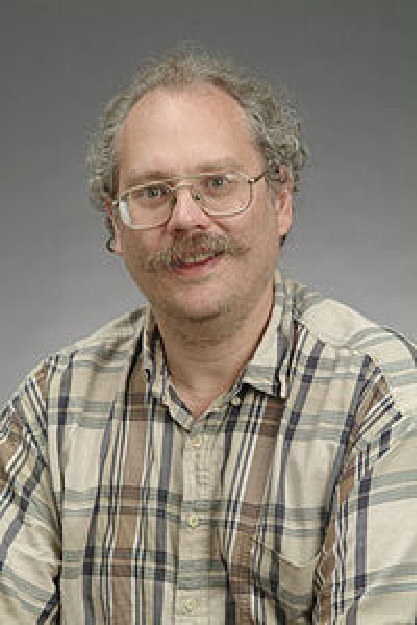
\includegraphics[scale=0.5]{shor.pdf}
\end{center}
}

% % % % % % % % % % % % % % 

\frame{
\frametitle{Задача о скрытой подгруппе}
% TODO Задача о скрытой подгруппе
\begin{itemize}
 \item У нас есть группа G, она имеет подгруппу H. 
 \item 
 \begin{defin}
  $f: G \to X$ -- прячет подгруппу H, если $\forall g_1,g_2 \in G: f(g_1) = f(g_2) \Leftrightarrow g_1H=g_2H$
 \end{defin}
\end{itemize}

\begin{astat}
 \textbf{Задача о скрытой подгруппе} --  задача о восстановлении образующих элементов подгруппы по отображению,  которое принимает  одинаковые значения на всех (левых) классах смежности относительно этой подгруппы. 
\end{astat}

\begin{stat}
 Алгоритм  Шора может эффективно решить HSP для конечных \textbf{абелевых} групп. 
\end{stat}




}

\frame{
\frametitle{Ну и ЧО?}
\begin{astat}
  Большинство специалистов сходятся во мнении, что достаточно стойкие симметричные шифры останутся стойкими и в квантовой модели вычислений
\end{astat}

\begin{astat}
 \textbf{Коммутативные и локально-коммутативных шифры} в опасности. Под этот случай подпадают схема Месси-Омуры, схема направленной подписи, система шифрования Эль-Гамаля, схемы груповой и слепой подписей и т.д. 
\end{astat}
\begin{astat}
 Ничего толком не известно про неабелевый случай.
\end{astat}


}


% % % % % % % % % % % % % % 
\frame{
% Все люди от природы стремятся к знанию. Доказательство тому — влечение к чувственным восприятиям: ведь независимо от того, есть от них польза или нет, их ценят ради них самих, и больше всех зрительные восприятия, ибо видение, можно сказать, мы предпочитаем всем остальным восприятиям, не только ради того, чтобы действовать, но и тогда, когда мы не собираемся что-либо делать. И причина этого в том, что зрение больше всех других чувств содействует нашему познанию и обнаруживает много различий [в вещах].
\frametitle{List of QC simulators}
\begin{itemize}
 \item http://www.quantiki.org/wiki/List\_of\_QC\_simulators
 \item curl, grep, sort -u, wc -l, немного магии...
 \item 95
 \item ??????
 \item PROFIT
\end{itemize}

}

\newcommand {\Exp} {\mathit{t}}
\newcommand {\Const} {\mathit{c}}
\newcommand {\Var} {\mathit{x}}

\frame{
\frametitle{Квантовое лямбда-исчисление}
% \resizebox{.1\hsize}{!}{
% \resizebox{0.7\hsize}{!}{%
% \begin{align*}
% \resizebox{0.7\hsize}{!}{
% \begin{array}{llll}
% \scalebox{0.7}{%
\begin{align*}
\Exp ::= &{}  &&\textbf{terms:} \\
      &\Var\  &&\textit{variable} \\
      &(\lambda \Var.\,\Exp)\   &&\textit{abstraction}   \\
      &(\Exp\ \Exp)  &&\textit{application} \\
      &\Const  &&\textit{constant} \\
      &!\Exp &&\textit{nonlinear term}\\
      &(\lambda !\Var.\,\Exp)\   &&\textit{nonlinear abstraction}   \\
\Const ::= &{} &&\textbf{constants:} \\
     &0\ |\ 1\ |\ \Had\ |\ \phase\ |\ \R\ |\ \cnot\ |\ \X\ |\ \Y\ |\ \Z\ |\ \dots
\end{align*}    
% }
% v ::= &{} &&\textbf{values:} \\
%       &x &&\textit{variable} \\
%       &\Const &&\textit{constant} \\
%       &(\lambda x.\,\Exp) &&\textit{linear abstraction} \\
%       &(\lambda !x.\,\Exp) &&\textit{nonlinear abstraction} \\
%       &!\Exp &&\textit{$!$-suspension}   
% \end{array}

% \resizebox{0.7\hsize}{!}{
%     $
%     \begin{array}{l}
%       p_1(x)=a_0+a_1x+a_2x^2 \\
%       p_2(x)=b_0+b_1x+b_2x^2+b_3x^3 \\
%       p_3(x)=c_0+c_1x+c_2x^2+c_3c^3+c_4x^4
%     \end{array}$%
%   }
% \resizebox{0.7\hsize}{!}{$
%   \Exp ::= &{}  &&\textit{terms:} \\
%       &\Var\  &&\textit{variable} \\
%       &(\lambda \Var.\,\Exp)\   &&\textit{abstraction}   \\
%       &(\Exp\ \Exp)  &&\textit{application} \\
%       &\Const  &&\textit{constant} \\
%       &!\Exp &&\textit{nonlinear term}\\
%       &(\lambda !\Var.\,\Exp)\   &&\textit{nonlinear abstraction}   \\
%   \Const ::= &{} &&\textit{constants:} \\
%     &0\ |\ 1\ |\ \Had\ |\ \phase\ |\ \R\ |\ \cnot\ |\ \X\ |\ \Y\ |\ \Z\ |\ \dots
% v ::= &{} &&\textit{values:} \\
%       &x &&\textit{variable} \\
%       &\Const &&\textit{constant} \\
%       &(\lambda x.\,\Exp) &&\textit{linear abstraction} \\
%       &(\lambda !x.\,\Exp) &&\textit{nonlinear abstraction} \\
%       &!\Exp &&\textit{$!$-suspension}   
%     $}  
% \end{align*}

% }
% \rulefig{
% \begin{align*}
% \Exp ::= &{}  &&\textit{terms:} \\
%       &\Var\  &&\textit{variable} \\
%       &(\lambda \Var.\,\Exp)\   &&\textit{abstraction}   \\
%       &(\Exp\ \Exp)  &&\textit{application} \\
%       &\Const  &&\textit{constant} \\
%       &!\Exp &&\textit{nonlinear term}\\
%       &(\lambda !\Var.\,\Exp)\   &&\textit{nonlinear abstraction}   \\
% \Const ::= &{} &&\textit{constants:} \\
%     &0\ |\ 1\ |\ \Had\ |\ \phase\ |\ \R\ |\ \cnot\ |\ \X\ |\ \Y\ |\ \Z\ |\ \dots
% v ::= &{} &&\textit{values:} \\
%       &x &&\textit{variable} \\
%       &\Const &&\textit{constant} \\
%       &(\lambda x.\,\Exp) &&\textit{linear abstraction} \\
%       &(\lambda !x.\,\Exp) &&\textit{nonlinear abstraction} \\
%       &!\Exp &&\textit{$!$-suspension}  
% \end{align*}
% }

}


\frame{
\frametitle{Scheme simulator}
\begin{description}
  \item[Что?] Scheme
 \item[Где?] http://www.het.brown.edu/people/andre/qlambda/
 \item[Кто виноват?] André van Tonder.
\end{description}
}



\frame{
\frametitle{Maxima -- qinf}
\begin{description}
  \item[Что?] Maxima
 \item[Где?] http://www.johnlapeyre.com/qinf/
 \item[Кто виноват?] G. John Lapeyre, Jr.
\end{description}
}


% \frame{
% 
% \frametitle{Scheme simulator}
% 
% }
% 
% \frame{
% 
% \frametitle{Scheme simulator}
% 
% }

\frame{
\frametitle{QIO -- Quantum IO Monad }
\begin{description}
  \item[Что?] Haskell
 \item[Где?] http://hackage.haskell.org/package/QIO
 \item[Кто виноват?] Alexander S. Green
\end{description}

}



\frame{
\frametitle{Quipper}
\begin{description}
  \item[Что?] \sout{Haskell} Quipper
 \item[Где?] http://www.mathstat.dal.ca/~selinger/quipper/
 \item[Кто виноват?]  Peter Selinger
\end{description}

}


% \frame{
% 
% \frametitle{QIO -- Quantum IO Monad }
% 
% }
% 
% \frame{
% 
% \frametitle{QIO -- Quantum IO Monad }
% 
% }




% % % % % % % % % % % % % % 
\frame{
\frametitle{Влияние -- квантовая связь}
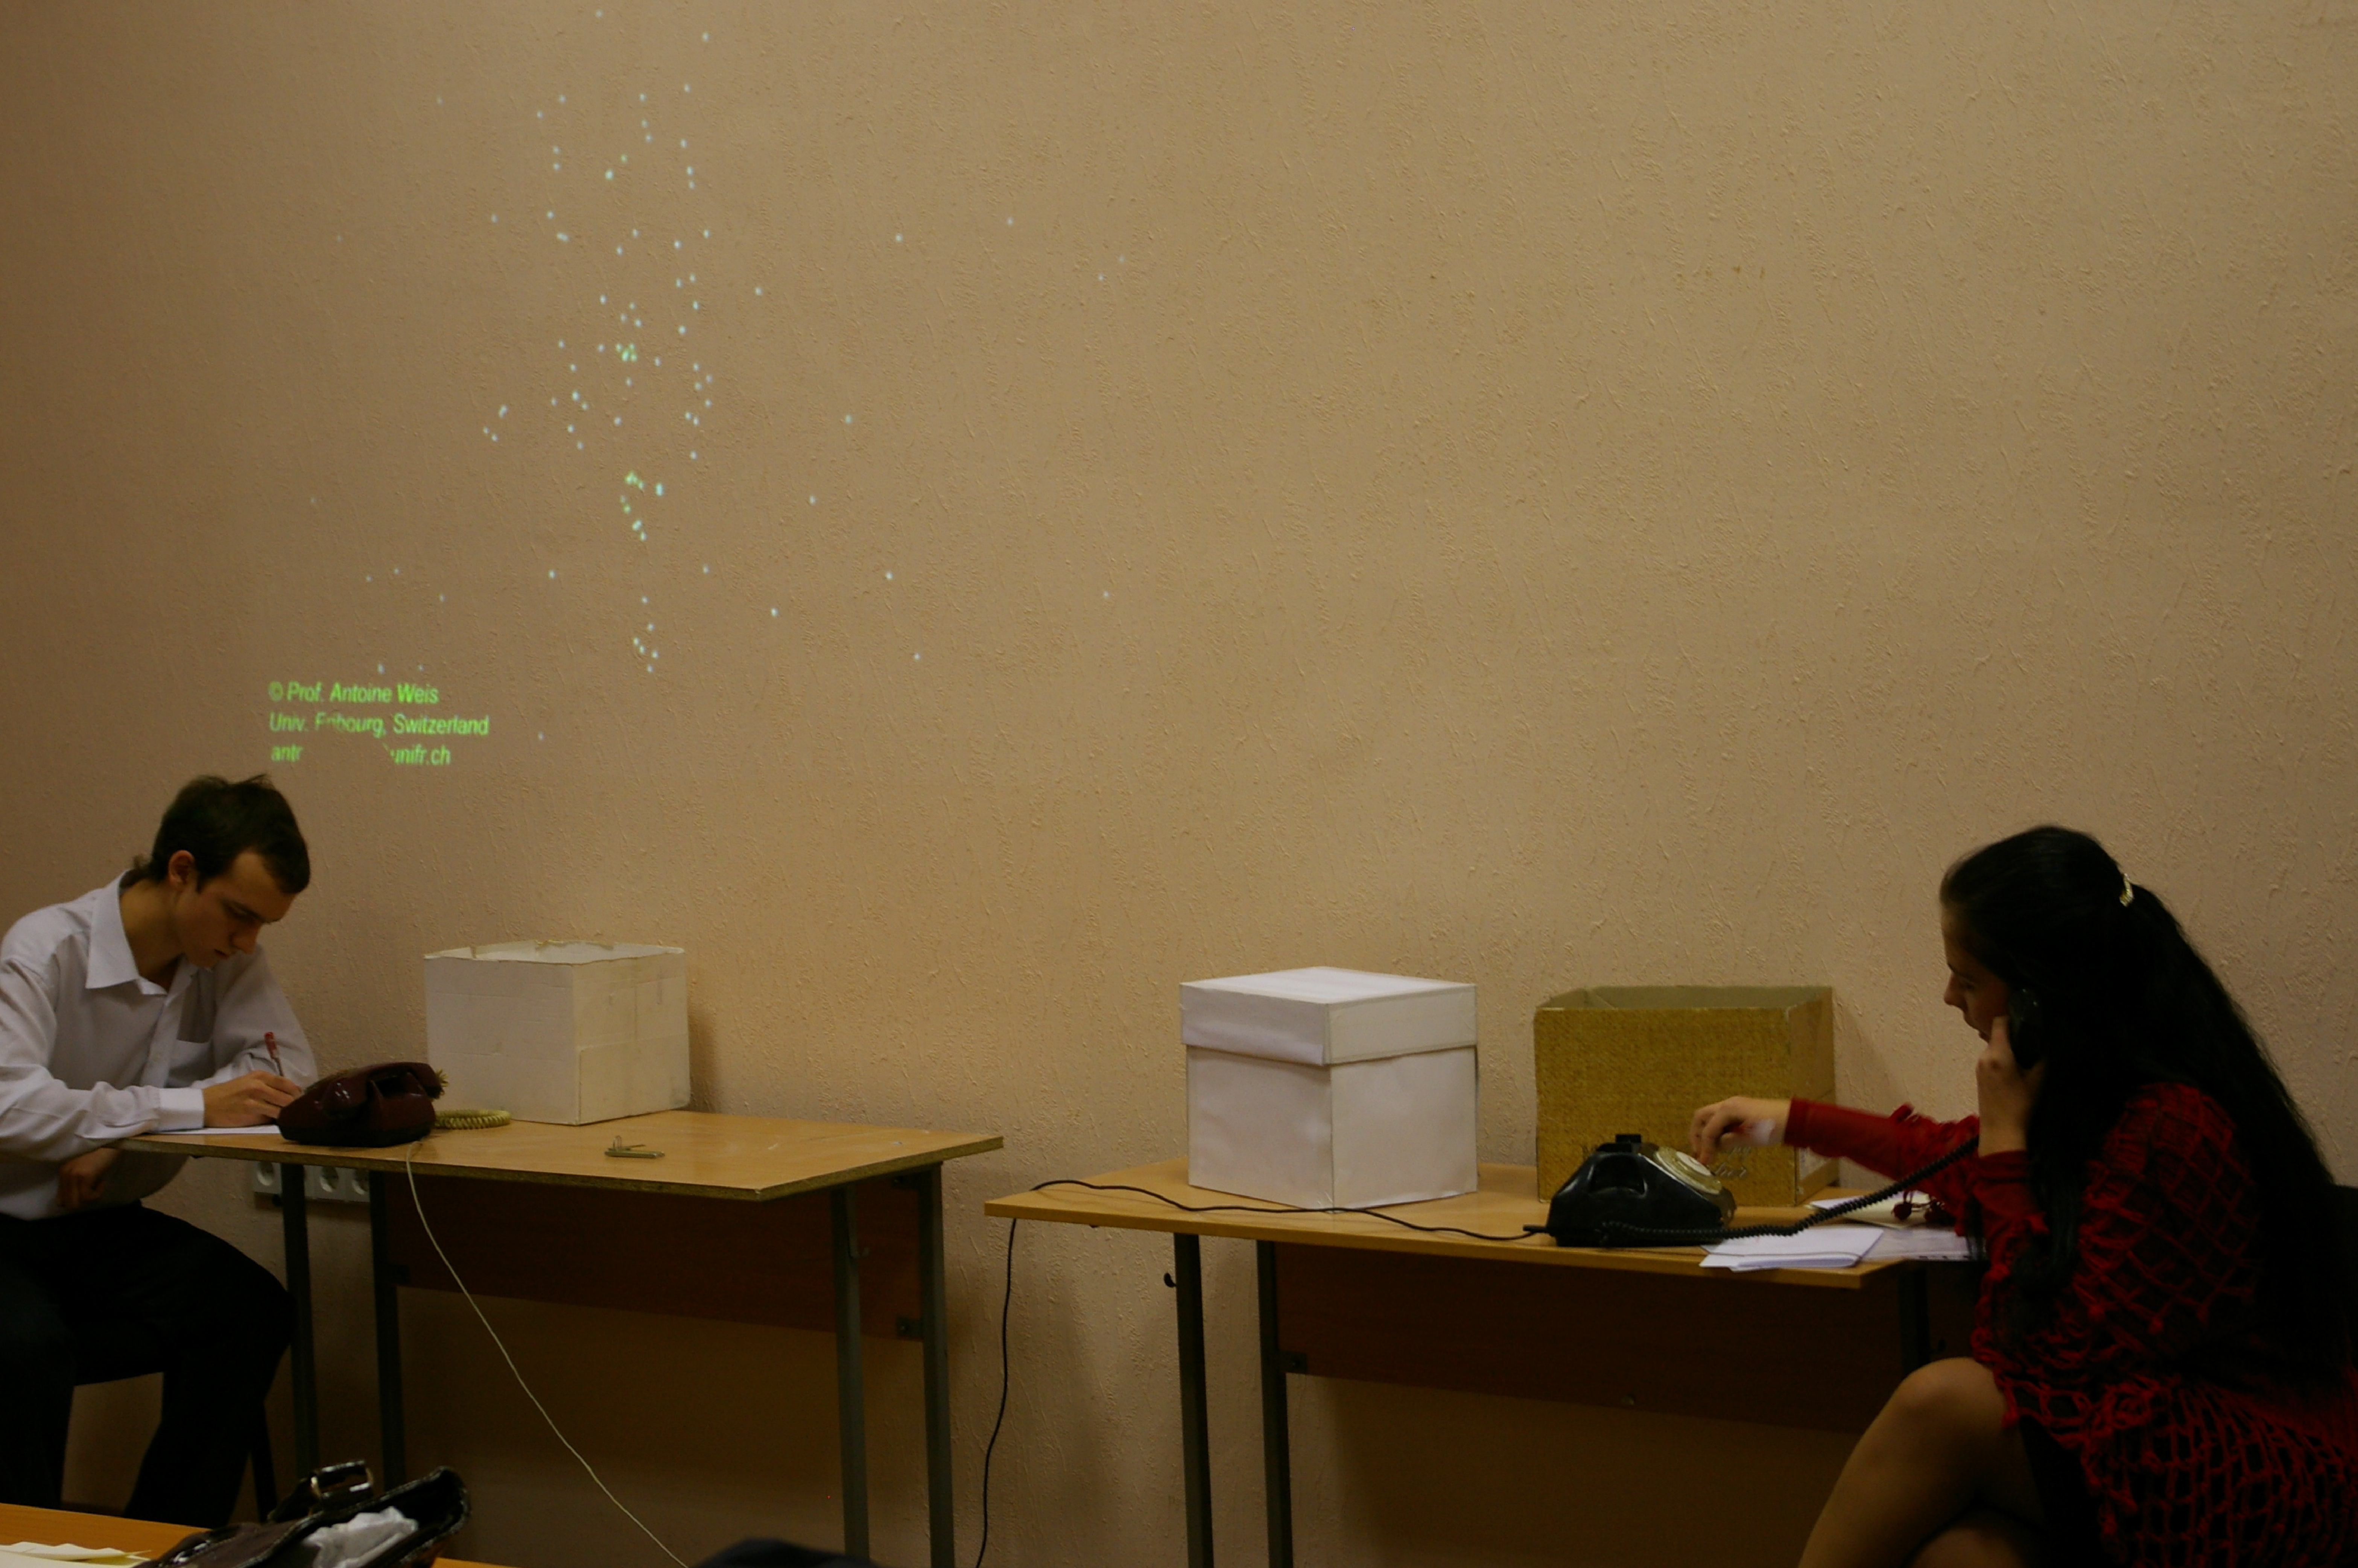
\includegraphics[scale=0.1]{qp0.pdf}
}

\frame{
\frametitle{Влияние -- квантовая связь}
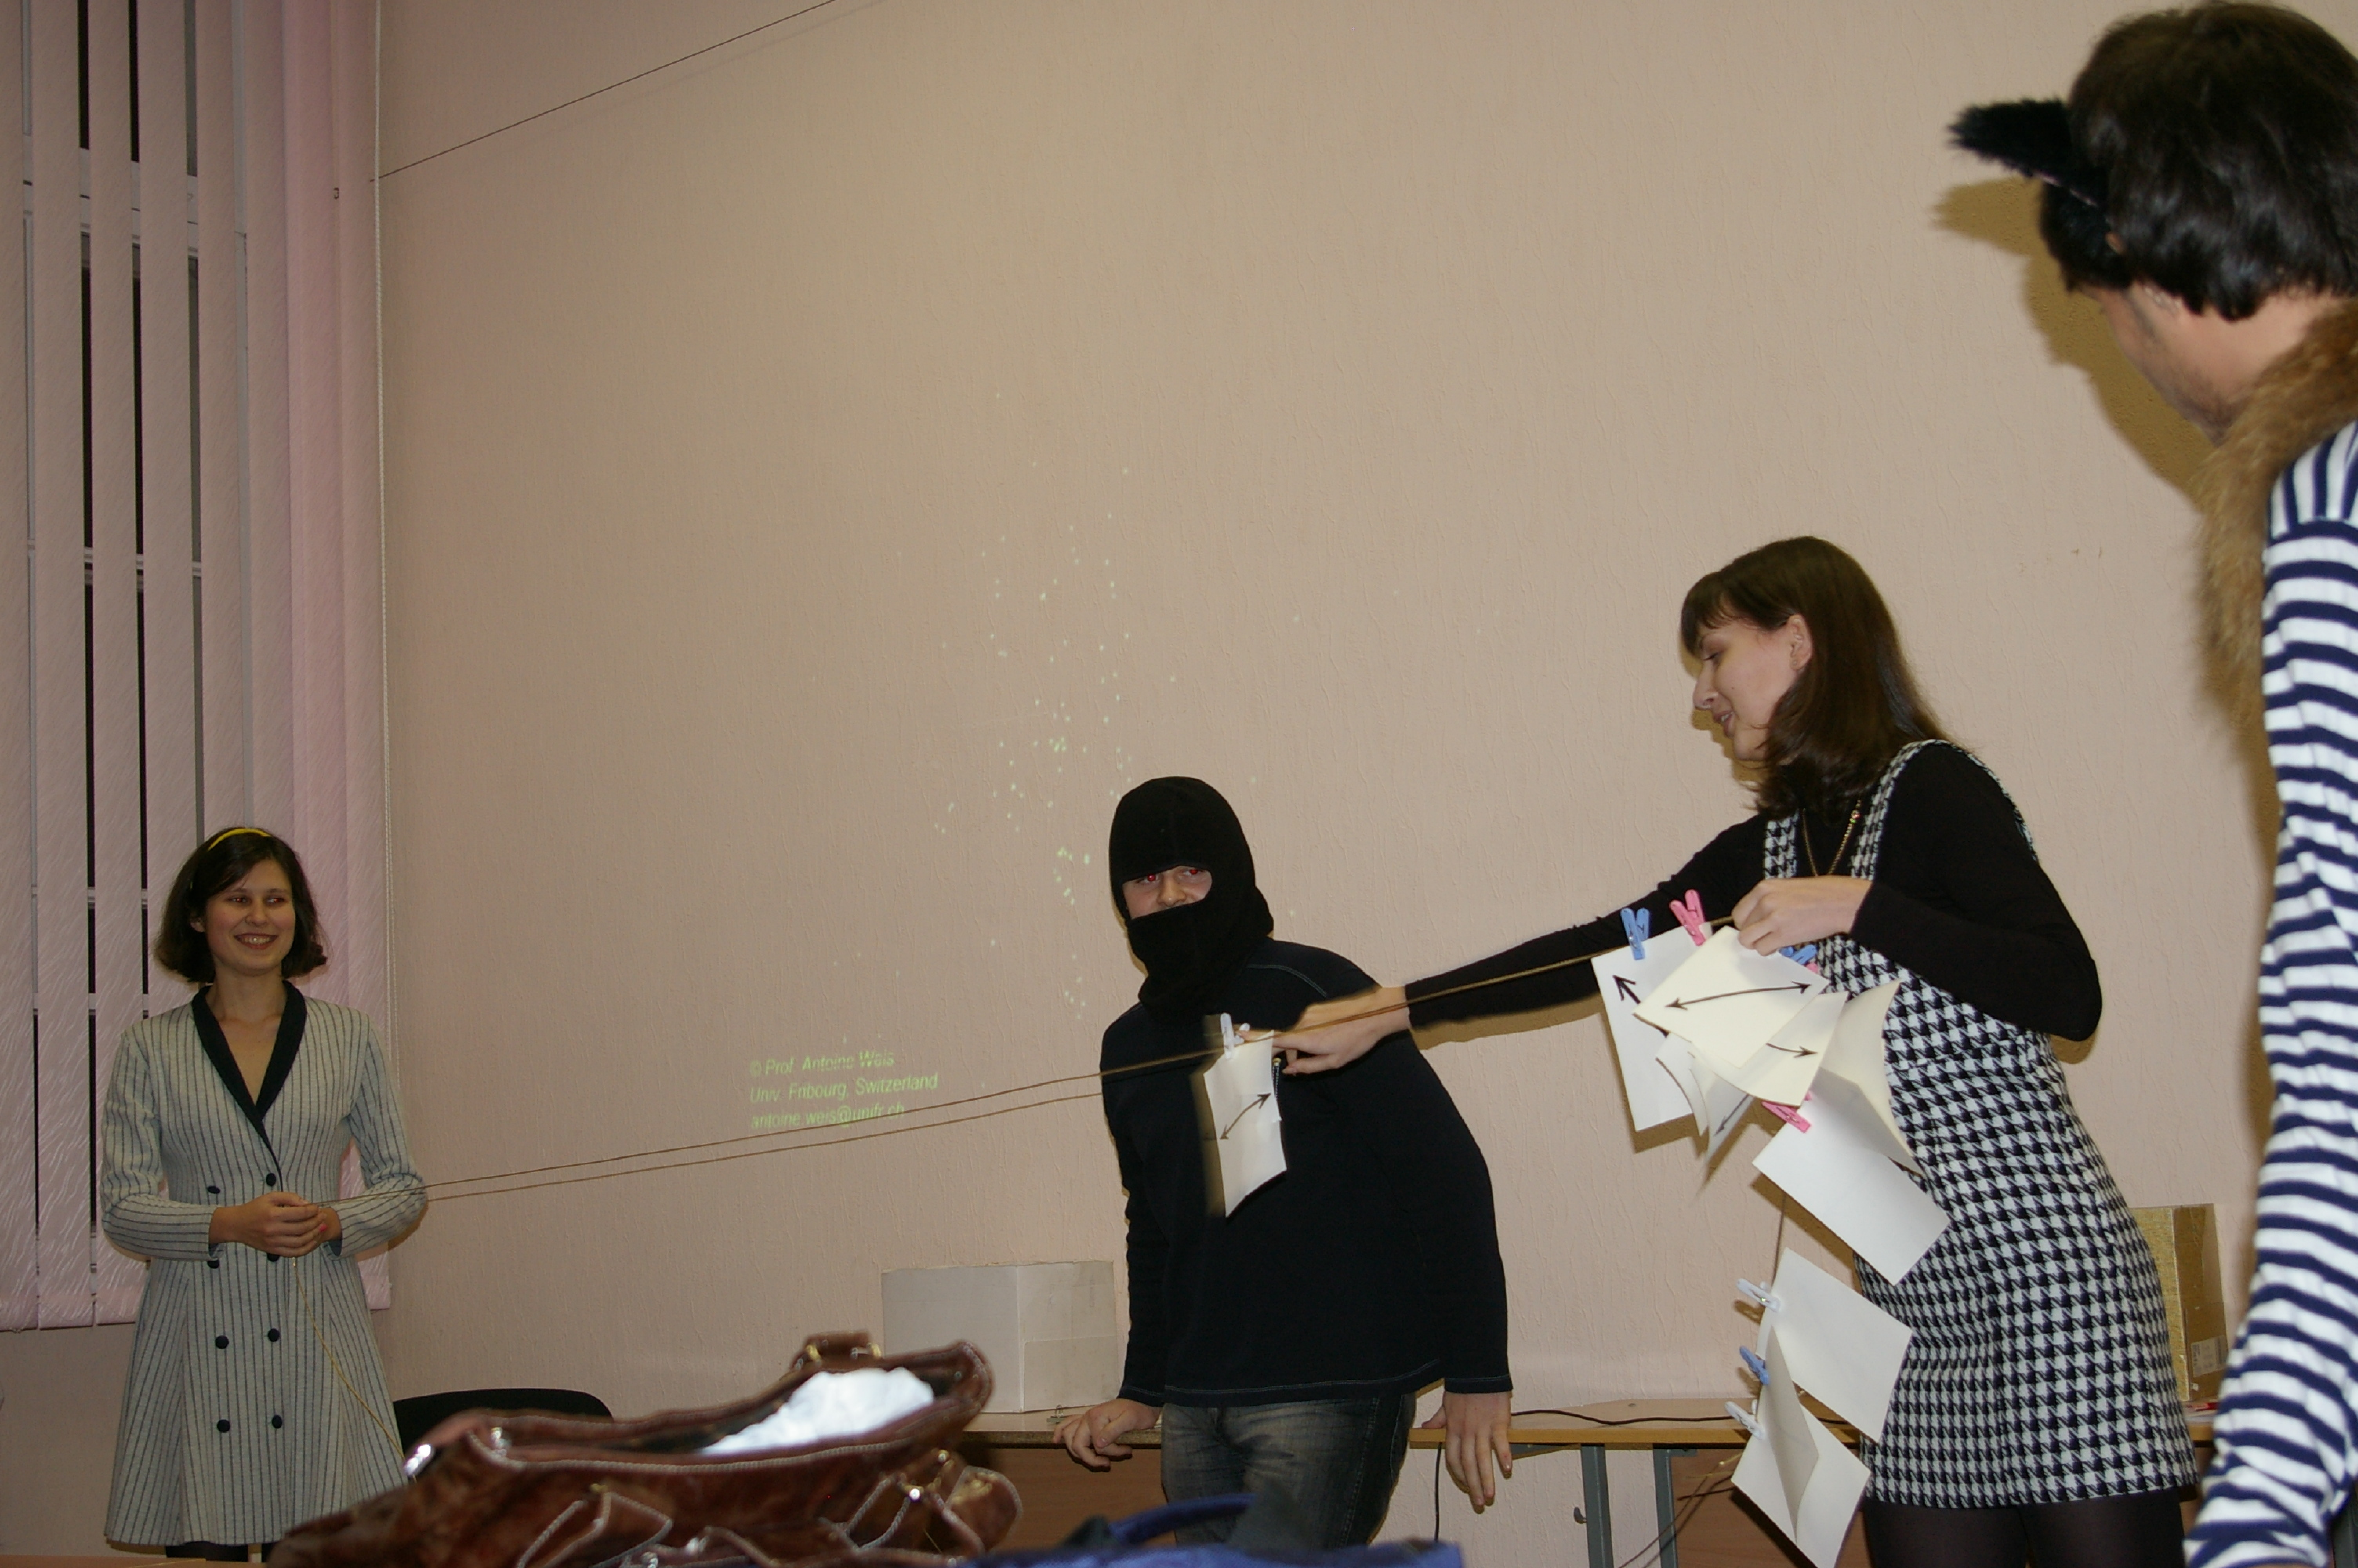
\includegraphics[scale=0.1]{qp1.pdf}
}

\frame{
\frametitle{Влияние -- квантовая связь}
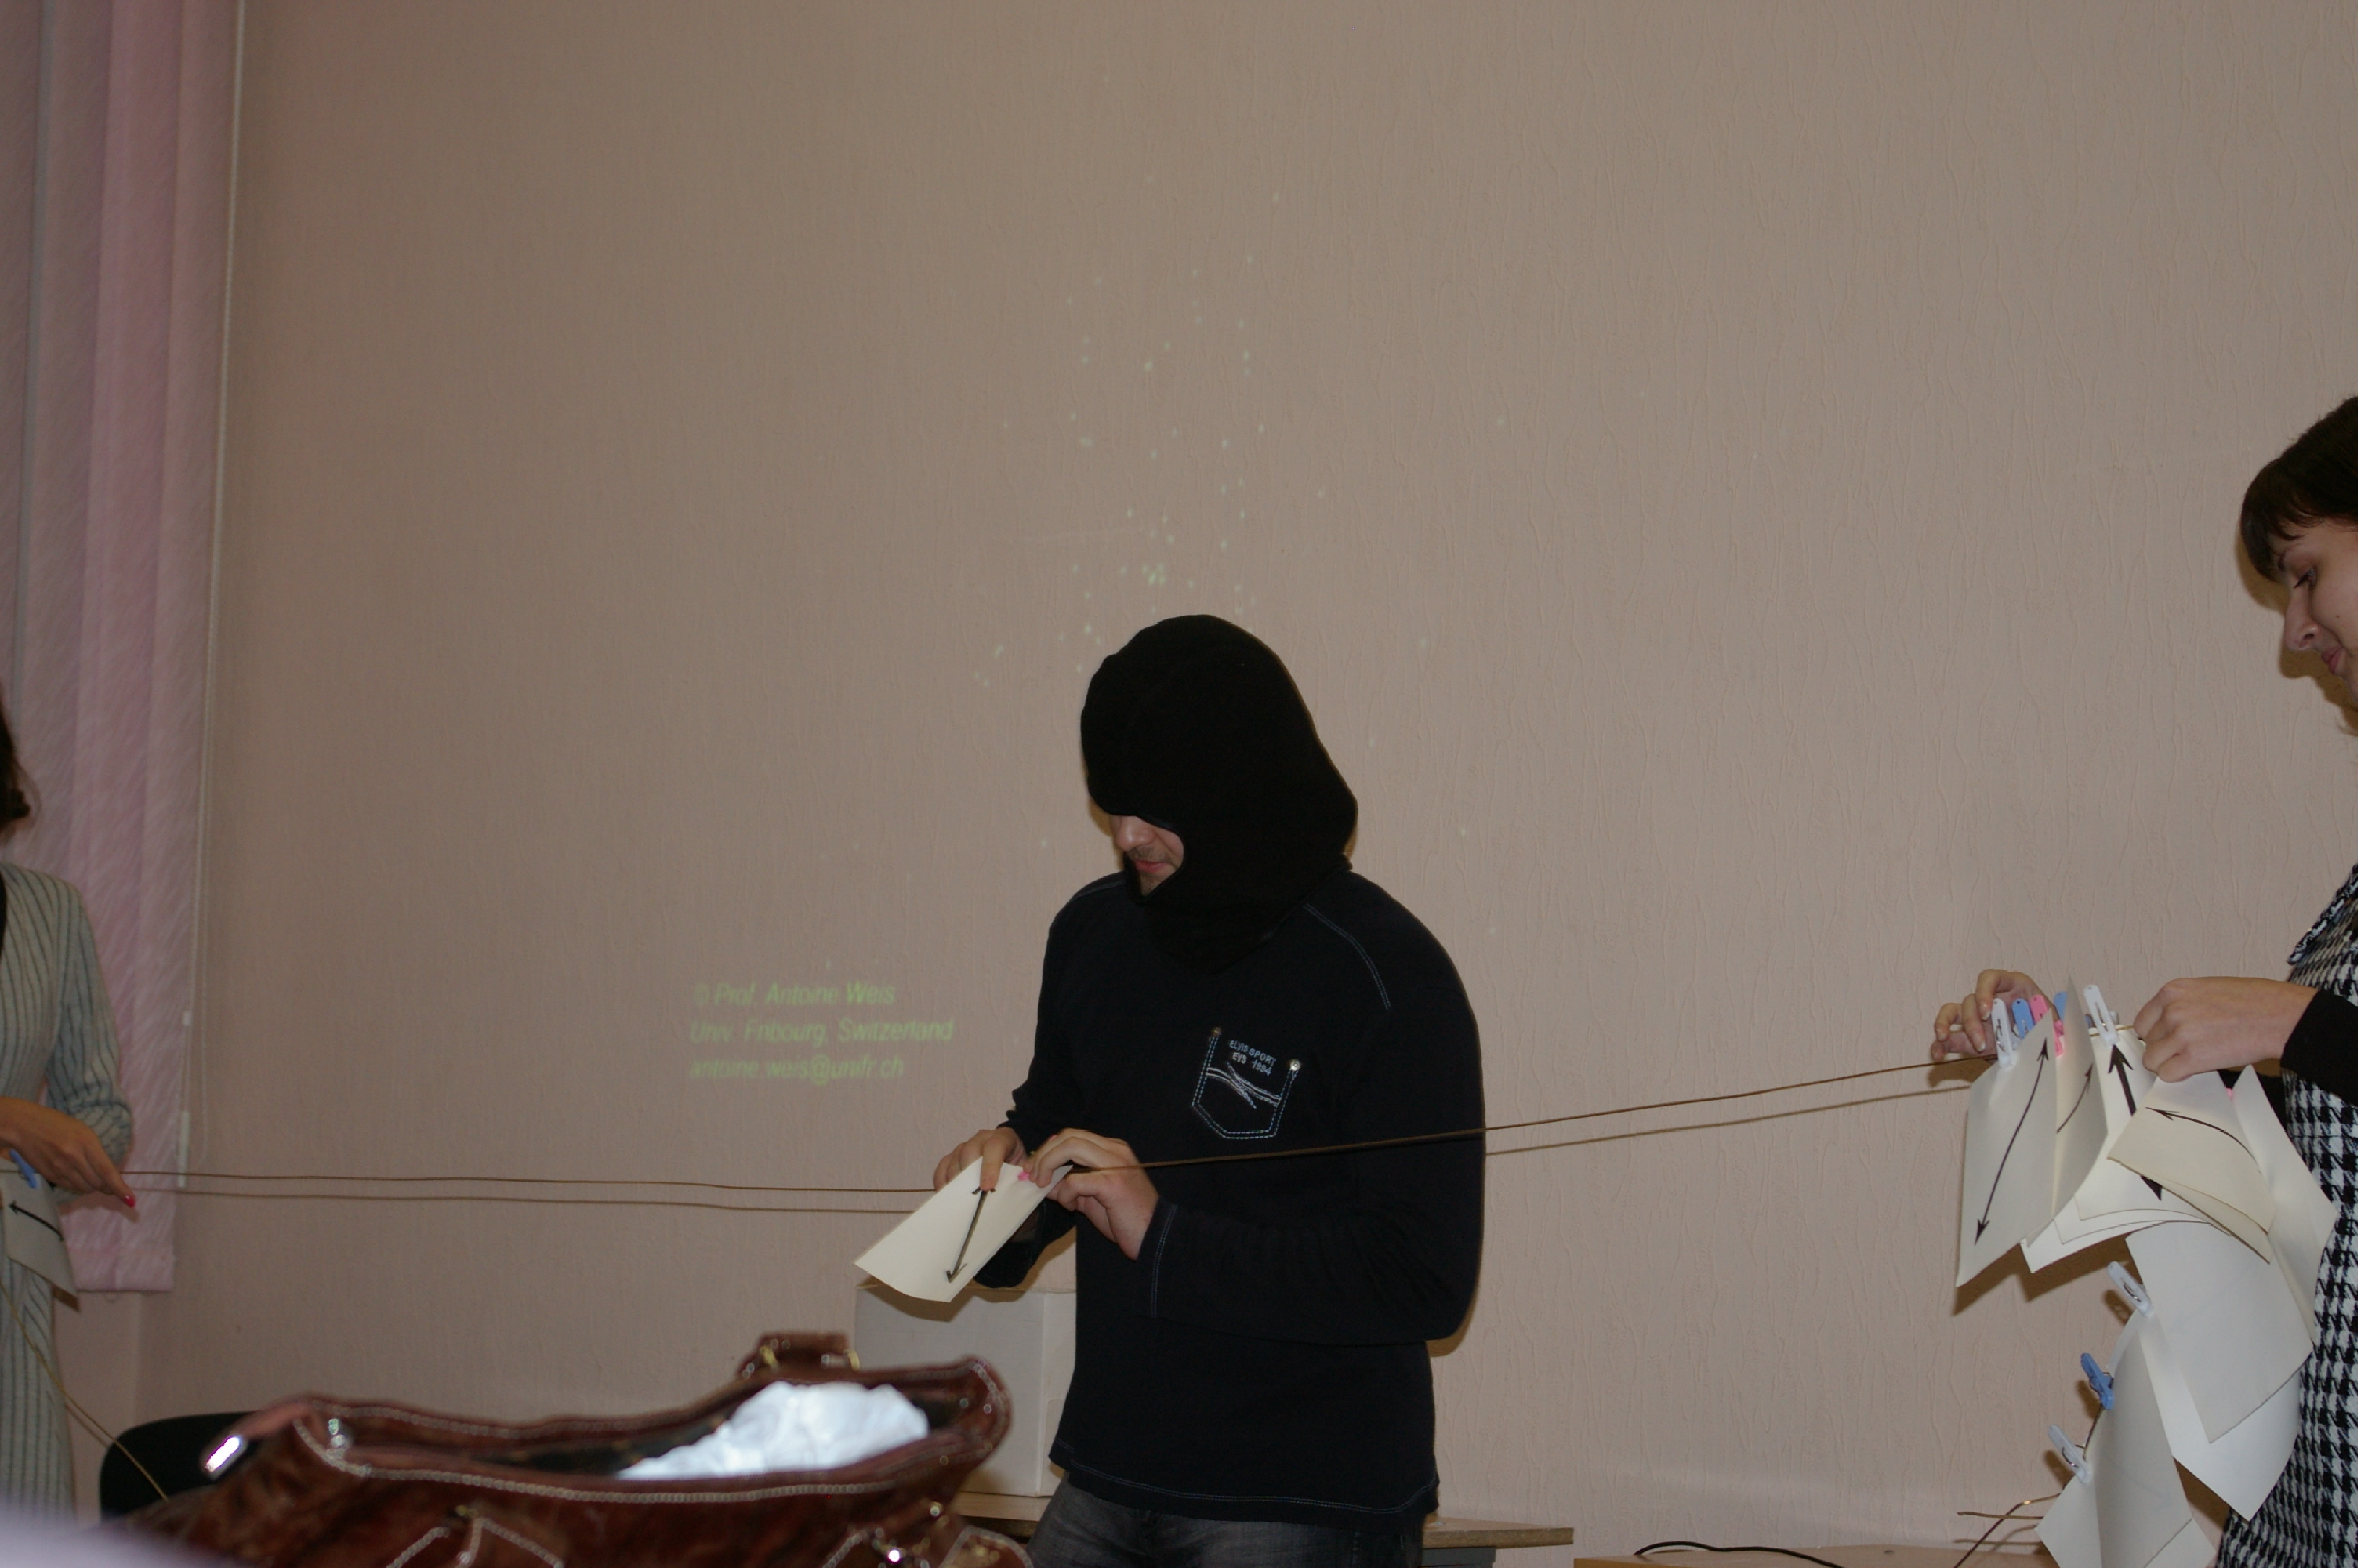
\includegraphics[scale=0.1]{qp2.pdf}
}

\frame{
\frametitle{Влияние -- цифровая физика}
Широко известные не в столь узких кругах обсуждения ``информационных'' аспектов физики:
\begin{itemize}
 \item Konrad Zuse \textit{Rechnender Raum}\footnote{Вычислительное пространство} (1967)
\item Lloyd, S., \textit{Programming the Universe: A Quantum Computer Scientist Takes On the Cosmos} (2006)
\item Хокинг, Прескилл,Сасскинд  и срачик о термодинамике черных дыр, которые ``теряют'' информацию.

\end{itemize}

}

\frame{
\frametitle{Влияние -- цифровая физика}
Интерпретации квантовой механики:
\begin{enumerate}
 \item Копенгагенская
\item Многомировая
\item Теории скрытого параметра(Schrödinger, Bohmian Mechanics )
\end{enumerate}
\begin{center}
\large В чем же разница? 
\end{center}

}

\frame{
\frametitle{Влияние -- цифровая физика}
Интерпретации квантовой механики:
\begin{enumerate}
 \item Копенгагенская
\item Многомировая
\item Теории скрытого параметра(Schrödinger, Bohmian Mechanics )
\end{enumerate}
\begin{center}
\large В чем же разница? 



\Huge РАЗНЫЕ ВСЕЛЕННЫЕ!

\normalsize
с разными вычислительными ресурсами!
\end{center}


}

\frame{
\frametitle{Влияние -- матан}
\begin{astat}
   We should expect a mathematical question to have a definite answer, if and only if we can phrase
the question in terms of a physical process we can imagine.
\end{astat}



David Deutsch



Новые математические методы, придуманые, пока возились с КК, можно использовать и в мирной жизни:
\begin{enumerate}
 \item $\epsilon$-approximating polynomials for symmetric functions
\item Robust polynomials
\item Lower bounds on locally decodable codes
\end{enumerate}

}

% \frame{
% 
% \frametitle{Влияние -- теория эволюции}
% 
% }


\frame{
\frametitle{Влияние -- теория сознания}
\begin{astat}
If we want a machine to be intelligent, it can't also be infallible. There are theorems that say almost exactly that.
 
\end{astat}
Turing

\begin{enumerate}
 \item Consciousness is reducible to computation (Strong-AI)
 \item Consciousness can be simulated by a computer, but the simulation couldn't produce "real understanding" (John Searle)
 \item Consciousness can't even be simulated by computer, but nevertheless has a scientific explanation (Penrose)
 \item Consciousness doesn't have a scientific explanation at all  (99\% \sout{хомячков} населения)
\end{enumerate}
%  Prof. Martin Plenio, Universität Ulm
% Abstract: In this lecture I will introduce some of the questions that we may wish to answer in quantum biology. Then I will focus on excitation energy transport in photosynthetic complexes. I will explain the crucial role of the interplay of quantum coherent evolution with environmental noise and provide an explanation of the origin and nature of the long-lived coherences that have been observed in the recent 2-D spectroscopy experiments of the FMO complex.
}

% \frame{
% \frametitle{Влияние -- теория сознания}
% 
% }


\frame{
\frametitle{Аналитическая машина}
\begin{center}
 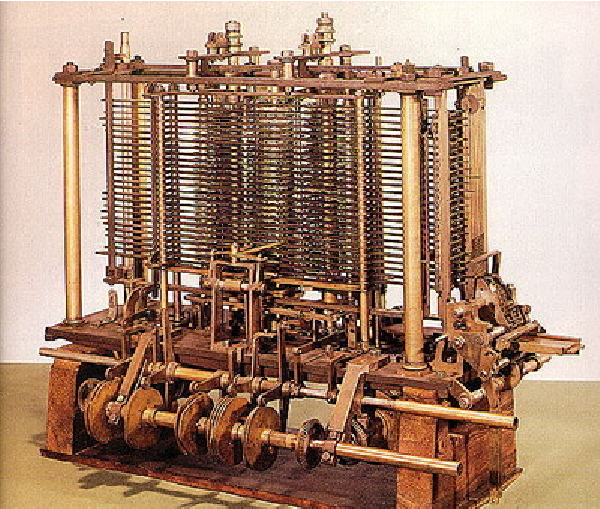
\includegraphics[scale=0.8]{de.pdf}

\end{center}

}





% % % % % % % % % % % % % % 
\frame{
\frametitle{Что почитать?}
Книги/лекции:
\begin{itemize}
 \item \textbf{CS191x} Quantum Mechanics and Quantum Computation
 \item \textbf{Лекции} -- Preskill(Caltech), Vazirani(Berkeley), Watrous(Waterloo), ...
 \item \textbf{Reference textbook} -- Nielsen and Chuang, \textit{Quantum Computation and Quantum Information}\footnote{Нильсен М., Чанг И. \textit{Квантовые вычисления и квантовая информация}. Пер. с англ - М.: Мир, 2006. - 824с}
 \item А. Китаев, А. Шень, М. Вялый. \textit{Классические и квантовые вычисления.}
 \item MIT OCW 6.845 \textit{Quantum Complexity Theory} -- Scott Aaronson
 \item Scott Aaronson \textit{Quantum Computing Since Democritus}
 \item Feynman lectures on computation

\end{itemize}


}

\frame{
\frametitle{Что почитать?}
Статьи:
\begin{itemize}
 \item Feynman, R. P. (1982). \textit{"Simulating physics with computers"}. (Перепечетано в Feynman lectures on computation)
 \item \textit{Quantum annealing with more than one hundred qubits},  	arXiv:1304.4595 
 \item \textit{Physics, Topology, Logic and Computation: A Rosetta Stone},  	arXiv:0903.0340
 \item \textit{Quantum Proofs for Classical Theorems}, 10.4086/toc.gs.2011.002
 \item \textit{NP-complete Problems and Physical Reality},  quant-ph/0502072

\end{itemize}


}
% % % % % % % % % % % % % % 

\frame{
 \frametitle{Feci, quod potui, faciant meliora potentes}
\begin{center}
\Huge Dixi\end{center}
}



%%%%%%%%%%%%%%%%%%%%%%%%%%%%%%%%%%%%%%%%%%%%%%%%%%%

% \frame{
% \frametitle{}
% 
% \begin{figure}[ht]
%  \includemovie[
%  poster,
%  text={\small P vs NP}
% ]{0.5\linewidth}{0.5\linewidth}{pnp.mp4}
% \end{figure}
% }

\end{document}
